% BI2113 Ecology and Evolution -- revision notes (AI-generated from the 02-Eco-Evo vault)
% Build: latexmk -pdf EcoEvo_Revision.tex   (chapters live in parts/)
\documentclass[11pt,a4paper]{article}
\usepackage[margin=2.1cm]{geometry}
\usepackage[T1]{fontenc}
\usepackage{lmodern}
\usepackage{microtype}
\usepackage{amsmath,amssymb,mathtools}
\usepackage{booktabs,tabularx,longtable,array}
\usepackage{enumitem}
\usepackage[dvipsnames]{xcolor}
\usepackage[most]{tcolorbox}
\usepackage{pgfplots}
\pgfplotsset{compat=1.18}
\usepgfplotslibrary{groupplots}
\usetikzlibrary{arrows.meta,positioning,calc}
\usepackage{multicol}
\usepackage{titlesec}
\usepackage{fancyhdr}
\usepackage[colorlinks=true,linkcolor=NavyBlue,urlcolor=NavyBlue]{hyperref}

\setlist{itemsep=2pt,topsep=3pt}
\setlength{\parindent}{0pt}
\setlength{\parskip}{5pt}
\renewcommand{\arraystretch}{1.25}

\titleformat{\section}{\Large\bfseries\color{NavyBlue}}{\thesection}{0.7em}{}
\titleformat{\subsection}{\large\bfseries\color{NavyBlue!80!black}}{\thesubsection}{0.6em}{}
\titleformat{\subsubsection}{\normalsize\bfseries}{\thesubsubsection}{0.5em}{}

\pagestyle{fancy}
\fancyhf{}
\lhead{\small BI2113 Ecology \& Evolution: revision}
\rhead{\small\nouppercase{\leftmark}}
\cfoot{\thepage}

% ---------- boxes ----------
\tcbset{enhanced,breakable,boxrule=0.6pt,arc=2pt,left=6pt,right=6pt,top=4pt,bottom=4pt,
        fonttitle=\bfseries\small}
% the core idea of a section
\newtcolorbox{keyidea}[1][]{colback=NavyBlue!5,colframe=NavyBlue!70!black,title={Core idea#1}}
% a chain of reasoning: each step follows from the one before
\newtcolorbox{chain}[1][]{colback=ForestGreen!5,colframe=ForestGreen!60!black,title={Reasoning chain#1}}
% statement-style MCQ practice: claims with verdict + reason
\newtcolorbox{statements}[1][]{colback=Goldenrod!8,colframe=Goldenrod!70!black,title={Statement check#1}}
% common errors
\newtcolorbox{trap}[1][]{colback=BrickRed!5,colframe=BrickRed!70!black,title={Trap#1}}
% subjective answer skeleton
\newtcolorbox{longans}[1][]{colback=Plum!6,colframe=Plum!70!black,title={Long-answer skeleton#1}}
% numbers worth memorising
\newtcolorbox{numbers}[1][]{colback=gray!6,colframe=gray!60!black,title={Numbers and facts#1}}
% worked example
\newtcolorbox{worked}[1][]{colback=white,colframe=Cerulean!70!black,title={Worked example#1}}

% verdict tags for statement checks
\newcommand{\T}{\textbf{\color{ForestGreen!70!black}[True]}\ }
\newcommand{\F}{\textbf{\color{BrickRed}[False]}\ }
\newcommand{\PT}{\textbf{\color{Goldenrod!60!black}[Half-true]}\ }
\newcommand{\why}{\par\hspace*{1.2em}$\hookrightarrow$\ }

\newcommand{\dd}{\mathrm{d}}

\title{\Huge\bfseries Ecology and Evolution (BI2113)\\[4pt]
\Large Revision notes for reasoning-based MCQs and long answers}
\author{Built from the 02-Eco-Evo vault (EE01--EE10, exam prep, solved past papers)}
\date{November 2026}

\begin{document}
\maketitle
\thispagestyle{empty}

\begin{tcolorbox}[colback=NavyBlue!4,colframe=NavyBlue!70!black,title={How to use these notes}]
The exam has \textbf{20 MCQs} and \textbf{20 marks of written answers}. The MCQs are said to be
\emph{statement or reasoning based}: you will be given claims (``A because B'', ``which of the following follows'',
``which statements are true'') and must judge whether the logic holds. A memorised definition does not answer
such a question; knowing \emph{why} a result holds, \emph{under what conditions}, and \emph{what would break it} does.
So each section is written as an argument:
\begin{itemize}
\item \textbf{Core idea} boxes give the one thing to understand;
\item \textbf{Reasoning chain} boxes lay out the steps from assumptions to result, saying why each follows;
\item \textbf{Statement check} boxes list plausible claims with a verdict and the reason. Use them as MCQ practice: cover the verdict, decide, then read the reason;
\item \textbf{Trap} boxes name the slips that MCQ distractors are built from;
\item \textbf{Long-answer skeleton} boxes give the structure a full written answer needs;
\item \textbf{Numbers and facts} boxes hold the case-study numbers the instructor asks you to memorise.
\end{itemize}
Section~\ref{sec:toolkit} lists the reasoning moves that recur across the course. Section~\ref{sec:examples} catalogues
every example (where it comes from, what is seen, what it shows). The glossary of terms and the equation sheet follow
(Sections~\ref{sec:glossary} and~\ref{sec:equations}), then a mixed drill.

\textbf{Syllabus rule} (lecture 1, slide 18): the slides plus the \emph{mandatory} readings are examinable; the
``detailed'' readings and papers are not. Paper-level material appears here only where it explains a slide, and is
marked \emph{(background)}.
\end{tcolorbox}

\tableofcontents
\newpage

% ===================================================================
\section{A reasoning toolkit for the whole course}\label{sec:toolkit}
% ===================================================================

A statement-based MCQ usually tests one of a small number of reasoning moves. The same moves recur in every chapter, so
learn them once.

\begin{enumerate}
\item \textbf{Null model, then departures.} Exponential growth (``first law of population dynamics'') and
Hardy--Weinberg are both descriptions of a system with \emph{no forces acting}. They are not expected to be true; they are
the baseline. A claim like ``the exponential model is useless because nothing grows exponentially for long'' misreads
the role of a null model.

\item \textbf{Per-capita versus total.} Many traps swap a per-capita quantity for a total one: logistic per-capita rate is
highest at small $N$ but total growth peaks at $K/2$; type II survivorship is a constant \emph{proportion} dying, not a
constant number; synchrony lowers the \emph{fraction} of calves lost, not the number per day.

\item \textbf{Which parameter controls what.} Ricker: $r$ sets the type of dynamics, $K$ only rescales. L--V
predator--prey: prey equilibrium is set by predator traits ($H^*=m/ap$), predator equilibrium by prey growth ($P^*=r/p$).
Competition: winning depends on $\alpha$ as well as $K$ (Park). $R^*$: the lowest break-even level wins, not the fastest
grower.

\item \textbf{Necessary versus sufficient.} $\alpha_{12}\alpha_{21}<1$ is necessary, not sufficient, for coexistence.
Cutting phosphorus is necessary, not sufficient, for clearing a shallow lake. Selection is necessary for adaptive
evolution but not sufficient without heritability. Irreducibility is not sufficient for convergence of a Leslie matrix
(primitivity is needed).

\item \textbf{Failing to reject is not proving.} A non-significant $\chi^2$ does not prove HWE; ``no chaos found'' with a
one-lag model does not prove simple dynamics.

\item \textbf{Stable, unstable, neutral.} A stable equilibrium attracts (logistic $K$); an unstable one repels (Allee
threshold, saddle in competition, underdominance); a neutral one does neither (L--V cycles, HW allele frequency). Neutral
states are disturbed permanently by shocks and are structurally fragile.

\item \textbf{Feedback signs.} Multiply signs around a loop: positive $=$ reinforcing (eutrophication's internal loading,
vegetation--turbidity, Allee effect, passenger pigeon); negative $=$ balancing (density dependence). Reinforcing loops plus
limits give alternative stable states and hysteresis.

\item \textbf{Thresholds and hysteresis.} The same picture appears in lakes (fold), Allee effects with harvesting,
competitive priority effects, underdominance and the wildebeest tracking radius. Past a threshold, undoing the original
change is not enough.

\item \textbf{Proximate versus ultimate.} ``How does it work?'' versus ``why does it exist?''. Both apply to every trait;
they never compete.

\item \textbf{Individuals versus populations.} Selection acts on individuals and phenotypes; evolution is a change in a
population's allele frequencies; individuals do not evolve.

\item \textbf{The model is not the world.} A model showing the expected behaviour is not thereby correct (L--V cycles; one-lag
fits finding stability; real-valued $N$ allowing chaos). Simple low-dimensional projections can hide complex
high-dimensional objects.

\item \textbf{Effort versus outcome, index versus estimate.} Number of reserves is not number of tigers; a pugmark or scat index
is not a population estimate ($\hat N=C/\hat p$).
\end{enumerate}

\begin{trap}[: how distractors are usually built]
Reversed causation (``character displacement makes species more similar''), swapped indices ($\alpha_{12}$ as the effect
of 1 on 2), a true fact with the wrong reason (``wildebeest migrate because the plains are wetter''), over-strong
conclusions (``proves'', ``always'', ``only''), and family-versus-population confusion (Yule's 3:1).
\end{trap}

% ===================================================================
\section{Biology, ecological thinking and the wildebeest (EE01)}
% ===================================================================

\subsection{Why biology resists a few neat equations}
Lecture 1 opens with three complaints: biology needs a lot of memorising, it is description-heavy, and it seems
to have no structure of ``a few equations from which the rest can be derived''. The answer the course gives is not
a defence of biology but a description of what biological systems are like. Slide 15 lists four features:

\begin{enumerate}
\item \textbf{Diversity and interconnectedness}, within a level (many species in one community) and across levels
(a change in a muscle protein can change a herd; a herd can change a river).
\item \textbf{Stochasticity}: which calf is caught, which seed lands where, which mutation arises.
\item \textbf{Historicity}: the present state depends on the particular path that produced it.
\item \textbf{Emergence}: properties of the whole are not found by dissecting the parts (``reductionism often fails'').
\end{enumerate}

\begin{chain}[: from the four features to the course's method]
Each feature blocks the physicist's route in its own way.
\begin{itemize}
\item Interconnectedness $\Rightarrow$ there is no isolated ``system'' to write equations for, and cutting a
system off from its connections changes how it behaves.
\item Stochasticity $\Rightarrow$ even a correct model predicts only probabilities.
\item Historicity $\Rightarrow$ the ``initial conditions'' are themselves a historical fact that has to be described,
not derived.
\item Emergence $\Rightarrow$ the behaviour of the whole cannot be assembled from the laws of the parts.
\end{itemize}
Therefore (slide 16): \textbf{mathematical formulation is typically difficult}, and when it can be done
\textbf{the relation with reality is statistical and conditional}. Two responses are possible: describe what is
there, or build simplified models with caveats. BI2113 uses (1) \emph{oversimplified mathematical models},
(2) \emph{a focus on concepts}, (3) \emph{historical narrative}, (4) \emph{examining the pedagogy}, and
accepts a trade-off: \textbf{breadth over depth}.

This also answers the three complaints: memorising and description come from diversity and history; the lack of
structure comes from mathematics working only locally, with caveats, while concepts and narrative carry the
connecting threads.
\end{chain}

\begin{keyidea}
``Oversimplified'' is a method, not an apology. A model is judged by what it teaches, not by how realistic it is:
the logistic equation is wrong for every real population and still explains why populations level off. The
course's wrap-up lecture repeats this: \emph{never mistake your model for reality}, and a model that shows the
expected behaviour is not thereby the right model.
\end{keyidea}

\subsection{Levels of organisation and the domain of the course}
Slide 13 draws a ladder: biomolecules $\to$ cells $\to$ tissues $\to$ organs $\to$ individual $\to$
population $\to$ community $\to$ ecosystem $\to$ biosphere. The levels from population upward change on
ecological time scales. \textbf{Changed trait values in a population are microevolution}; accumulated, they lead
through \textbf{speciation} to \textbf{macroevolution}. The individual's life cycle (meiosis to a gamete,
fertilisation to a cell) links the sub-organismal levels back to the individual. Slide 14 removes the
sub-organismal levels: \textbf{the domain of BI2113 is the individual and above}.

Different levels run on different clocks: muscle contraction in milliseconds, a migration in a year, the rise of a
lineage in millions of years. A model that follows one clock can treat the slower processes as fixed and the
faster ones as instantaneous. That separation of time scales is what makes simple models possible at all.

\subsection{Proximate and ultimate questions}
Slide 5 splits the wildebeest migration into \emph{how} and \emph{why}:
\begin{itemize}
\item \textbf{How} (proximate): the mechanism inside one individual now: physiology, development, cues, behaviour rules.
\item \textbf{Why} (ultimate): the benefit that made selection favour the trait; its evolutionary history.
\end{itemize}
Both kinds of answer apply to \emph{every} trait. They are not rival explanations; they answer different
questions. (Mayr's names for them, and his example of the warbler that migrates on day-length cues while the
screech owl in the same wood stays, are background reading.)

\begin{trap}
Confusing the \emph{mechanism} of synchronous calving with its \emph{benefit}. How females synchronise (a fall in
forage protein triggers the cycle; a silent first ovulation cues bulls and other females) is proximate. Why it pays
(swamping predators) is ultimate. ``Calves stand within 6 minutes'' is proximate; ``this lets them keep up with a
herd that must move'' is ultimate.
\end{trap}

\subsection{The wildebeest case}
\subsubsection*{How: three adaptations}
\begin{enumerate}
\item \textbf{Efficient muscle.} 62.6\,\% efficient, against 41.8\,\% (cow) and 34\,\% (mouse) (Curtin et al.\
2018). Efficiency $\eta$ is the fraction of chemical energy used that comes out as mechanical work; the rest is
heat. For work $W$ the fuel burnt is $W/\eta$ and the heat released is $W(1/\eta-1)$. A cow therefore needs
$0.626/0.418=1.50\times$ the fuel, but releases $1.39/0.60=2.3\times$ the heat. Heat is what is left over, so it
grows much faster than fuel as $\eta$ falls; in a hot, dry habitat, shedding heat costs water.
\item \textbf{Synchronous births.} About 250{,}000 calves in about three weeks from mid-February, roughly 80\,\% of the
year's calves: about 12{,}000 a day, 500 an hour. Predators with a limited capacity to chase, kill and eat cannot
take more than a fixed number per day, so concentrating births lowers the \emph{fraction} lost
(\textbf{predator satiation}).
\item \textbf{Precocial calves.} A calf stands in about 6 minutes and walks in 30; topi and hartebeest calves take
much longer. A herd that must keep moving cannot afford helpless young.
\end{enumerate}

\begin{chain}[: why synchrony protects calves (a bound)]
Let $N$ calves be born over $w$ days and let predators kill at most $K$ per day. Losses in the window are at most
$Kw$, so the fraction lost is at most $\min(1,\,Kw/N)$. Shortening $w$ lowers the cap in proportion, as long as
$K<N/w$. If the herd is small ($N/w<K$) there is no cap, and a pulse of births may even attract predators: synchrony
works only with large numbers.
\end{chain}

\subsubsection*{Why: opposing gradients}
Rainfall rises from the south-east short-grass plains ($\sim$400\,mm) to the north-west woodland ($\sim$1200\,mm),
but soil fertility and grass protein run the other way (the plains sit on nutrient-rich volcanic ash). The puzzle
the slide sets: if the woodland is wetter all year, why do herds go onto the dry plains at the start of the rains?

\begin{chain}[: why a migration, rather than staying put]
\begin{enumerate}
\item Rain controls \emph{how much} green grass exists; fertility controls \emph{how good} it is.
\item The two gradients are opposed, so no single place is best all year: the plains are best (protein-rich, short
grass) while the rains last; the woodland when the plains dry out.
\item An animal that compares sites over a large enough distance therefore keeps moving. In Holdo et al.'s
models (background), rules using intake combined with plant nitrogen fit the observed herd distribution far better
than rules using biomass alone, and a migration appears only when the tracking radius exceeds about 80--100\,km;
with only local comparisons the simulated herd gets trapped.
\end{enumerate}
So ``they follow the rain'' is incomplete: they follow \emph{quality}, and the migration is an emergent property of
many animals following a simple rule on a landscape with opposed gradients.
\end{chain}

\subsubsection*{What the migration does to the ecosystem}
\begin{itemize}
\item \textbf{Death}: annual mass drownings at the Mara River crossings (about 6{,}000 a year) are a recurring pulse of
food and nutrients for fish and scavengers; bones release phosphorus for years.
\item \textbf{Fire}: grazing removes fuel. After rinderpest was eradicated in the 1960s the herd surged, fire
declined and trees recovered (background: a virus-to-landscape trophic cascade).
\end{itemize}

\subsubsection*{Why so many? (Hopcraft, background but a model of reasoning)}
Wildebeest outnumber the next herbivore (zebra) about six-fold. The argument eliminates explanations by comparison:
against topi and hartebeest (biology helps but is not enough: wildebeest are not that dense elsewhere); against
resident wildebeest herds (same biology, 30--240$\times$ fewer: residents are \emph{habitat-limited}); against zebra
(also migratory but far fewer: probably \emph{predation-limited}). The general recipe for migratory
superabundance: \textbf{refuge areas, an ephemeral high-quality resource, and connectivity} between patches.

\begin{numbers}
$\sim$1{,}500\,km a year; herd $\approx$1.2--1.3 million; muscle 62.6\,\% (cow 41.8, mouse 34); 250{,}000 calves in
$\sim$3 weeks ($\approx$80\,\% of the year's); calf stands in $\sim$6 min; rain 400\,$\to$\,1{,}200\,mm SE$\to$NW;
tracking radius $\gtrsim$80--100\,km; $\sim$6{,}000 drownings a year.
\end{numbers}

\begin{statements}
\begin{enumerate}[label=\arabic*.]
\item ``Wildebeest migrate because the plains get more rain early in the season.''
\F The woodland is wetter all year. The pull of the plains is grass \emph{quality} (protein, on fertile soil).
\item ``Proximate and ultimate explanations of a trait compete; at most one can be right.''
\F They answer different questions (how vs why) and both apply to every trait.
\item ``Synchronous calving lowers the number of calves predators take per day.''
\F It lowers the \emph{fraction} taken: predators are saturated, so the number per day is capped while births
per day are huge.
\item ``Because the wildebeest muscle is 1.5$\times$ more fuel-efficient than the cow's, it also releases 1.5$\times$ less heat.''
\F Heat per unit work is $1/\eta-1$: 0.60 against 1.39, a factor of 2.3. The heat ratio is bigger than the fuel ratio.
\item ``If biological systems are stochastic, a model of them cannot be useful.''
\F Models then predict probabilities and trends; the relation with data is statistical and conditional, which is
still informative.
\item ``Removing 6{,}000 drownings a year would change the wildebeest population a lot.''
\F About 0.5\,\% of a food-limited herd; density dependence soon offsets it. The river ecosystem, which loses a
nutrient subsidy, changes far more (2025 end-sem Q11).
\end{enumerate}
\end{statements}

\begin{longans}[: ``Why is the wildebeest the dominant herbivore of the Serengeti?'']
(1) \emph{Biology}: grazing adaptations for short protein-rich grass; efficient muscle for long travel; synchronous,
precocial calving that swamps and outruns predators. (2) \emph{Environment}: opposed rainfall and fertility
gradients, so high-quality grass exists somewhere reachable all year if animals move over $\gtrsim$80\,km.
(3) \emph{Comparisons}: residents with the same biology are habitat-limited; zebra, also migratory, are
predation-limited. (4) \emph{General recipe}: refuge, ephemeral high-quality resource, connectivity. (5) Note the
two-way interaction: the herd changes fire regimes and river nutrients.
\end{longans}

% ===================================================================
\section{Structured populations: life tables, matrices, elasticity (EE02)}
% ===================================================================

\subsection{What a population is and what we ask of it}
\textbf{Ecology} (Haeckel, 1866; \emph{oikos} = house) is the study of interactions among organisms and their biotic
and abiotic environment, and how these lead to patterns of distribution and abundance. A \textbf{population} is a
group of similar individuals inhabiting a defined space at a given time. Population ecologists study
\textbf{distribution} (spread over space), \textbf{demography} (age structure, survivorship, birth rates) and
\textbf{dynamics} (how and why numbers change). Reasons to study non-human populations: conservation, management of
useful species, control of pests and invaders, and the population being the \textbf{unit of evolution}.

The population is a ledger: $N_{t+1}=N_t+B-D+I-E$. If every individual had the same per-capita rates, one number
would describe growth. This chapter asks what happens when \textbf{individuals are not interchangeable}: a newborn, a
breeder and an old animal survive and reproduce differently. That is \emph{population structure}.

\subsection{The cohort life table and $R_0$}
Follow a \textbf{cohort} (individuals born in the same period) to the last death. Columns: $n_x$ alive at the start of
class $x$; $l_x=n_x/n_0$ the proportion surviving to $x$; $m_x$ the mean offspring per survivor in class $x$; and
$l_xm_x$ the expected offspring per \emph{newborn} from that class. Summing gives the \textbf{net reproductive rate}
\[
R_0=\sum_x l_x m_x ,
\]
the mean number of offspring a newborn produces over its whole life. $R_0>1$: each generation larger than the last;
$R_0<1$: shrinking. \emph{Phlox drummondii} (annual plant, cohort of 996): $R_0=2.4177$. Its survival is front-loaded
(84\,\% die before day 299) and reproduction concentrated in a few late weeks.

Three ways to get survival data (Molles): \textbf{cohort} table (most reliable, impractical for long-lived or mobile
species); \textbf{static} table (ages at death of many individuals, e.g.\ Dall sheep skulls; assumes the death-age
distribution represents survival); \textbf{from an age distribution} (differences between classes; assumes a
stationary, closed population, so least accurate).

\begin{trap}
$R_0$ is a factor \emph{per generation}; $\lambda$ is a factor \emph{per time step}. They are equal only for
non-overlapping generations (an annual plant). In general they agree only on the threshold: $\lambda>1\iff R_0>1$.
\end{trap}

Unlimited growth at $\lambda=2.42$ would cover North America with $\sim$77 \emph{Phlox} per m$^2$ in 32 years:
natural populations have a huge capacity for increase, so something must change as $N$ grows (density dependence,
next section).

\subsection{Survivorship curves and the log axis}
\begin{chain}[: why survivorship is plotted on a log axis]
If an individual has the same probability $q$ of dying in every interval, then $n_{x+1}=(1-q)n_x$, so
$n_x=n_0(1-q)^x$ and
\[
\ln n_x=\ln n_0+x\ln(1-q).
\]
Constant per-capita risk is therefore a \textbf{straight line} on a log axis, with slope $\ln(1-q)$. Slide 12: 60\,\%
die each interval; numbers 1000, 400, 160, 64. The \emph{losses} shrink (600, 240, 96) but the \emph{proportion}
lost (and the log-slope) is the same each time. A log axis shows the risk to \emph{one individual}; a linear axis
shows the number of bodies. Population dynamics asks about per-capita rates, so the log axis is the right one.
\end{chain}

\begin{itemize}
\item \textbf{Type I}: low mortality until late in life (large mammals, humans; Dall sheep, \emph{Phlox} after its
first period).
\item \textbf{Type II}: constant proportion dies per interval; straight line on a log axis (many birds: robin,
white-crowned sparrow).
\item \textbf{Type III}: very high juvenile mortality, then high survival (marine fish, mackerel; the desert shrub
\emph{Cleome}).
\end{itemize}
The idealised types are \emph{bounds} on what is possible; real curves are mixtures (\emph{Phlox}: a Type III-like
early loss, a plateau, then a Type I-like end).

\begin{trap}
A steep early drop (Type III) says nothing about lifespan: the survivors may live long. And the slope on a log axis is
the per-capita hazard, not the number of deaths.
\end{trap}

\subsection{The Leslie matrix: age structure with births}
A cohort table ignores the cohort's children. To project the whole population, count every age class and let births
join class 1:
\[
\begin{pmatrix}n_1\\n_2\\n_3\\n_4\end{pmatrix}_{t+1}=
\begin{pmatrix}F_1&F_2&F_3&F_4\\P_1&0&0&0\\0&P_2&0&0\\0&0&P_3&0\end{pmatrix}
\begin{pmatrix}n_1\\n_2\\n_3\\n_4\end{pmatrix}_{t}.
\]
Row 1 reads ``babies = $\sum$ fecundity $\times$ number in each class''; each sub-diagonal row reads ``class $x+1$ =
survivors of class $x$''.

Slide 16: $P=(0.5,0.2,0.1)$, $F=(0,2,1,1)$, start with 200 newborns. The totals first zig-zag
(200, 100, 220, 122, 232, \dots) because one cohort breeds in pulses; then
\begin{itemize}
\item the total grows \textbf{geometrically} by $\lambda=1.05082$ per step (slide 18, 20);
\item the age \emph{proportions} settle at $(0.635,\,0.302,\,0.057,\,0.005)$: the \textbf{stable age distribution}
(SAD), even though the numbers keep growing (slide 19).
\end{itemize}

\begin{chain}[: why the population settles (eigenvalues)]
\begin{enumerate}
\item Try a solution in which every class grows by the same factor: $\mathbf n_t=\lambda^t\mathbf w$. Then
$\mathbf A\mathbf w=\lambda\mathbf w$: $\lambda$ is an eigenvalue and $\mathbf w$ its eigenvector.
\item Any start is a sum of such modes, $\sum_i c_i\lambda_i^t\mathbf w_i$. After many steps the mode with the
largest $|\lambda_i|$ dominates; the others shrink \emph{relative to it} like $(|\lambda_i|/\lambda_1)^t$.
\item So the shape converges to $\mathbf w_1$ (the SAD) and the growth ratio to $\lambda_1$, \emph{whatever the
starting mix}. The matrix ``forgets'' its start (ergodicity). The SAD depends only on the vital rates, not the initial
vector.
\item The sub-diagonal rows give $w_{x+1}/w_x=P_x/\lambda$, and the first row gives the discrete Euler--Lotka equation
\[
1=\sum_x F_x\,l_x\,\lambda^{-x}.
\]
Its right side falls steadily as $\lambda$ rises, so it has one positive root; at $\lambda=1$ it equals $R_0$. Hence
$\lambda>1\iff R_0>1$.
\end{enumerate}
\end{chain}

\textbf{Perron--Frobenius.} The slide states that a non-negative matrix has a real dominant eigenvalue. For
convergence to a fixed shape the matrix must be non-negative, \textbf{irreducible} (life-cycle graph connected) and
\textbf{primitive} (the loop lengths have greatest common divisor 1). Then $\lambda_1$ is real, positive, simple and
strictly larger in modulus than every other eigenvalue, and $\mathbf w$ (SAD) and $\mathbf v$ (reproductive values)
are strictly positive.

\begin{trap}
A species that reproduces in only \emph{one} age class (semelparous, single loop) gives an \emph{imprimitive} matrix:
e.g.\ $F_3=6$, $P_1=0.5$, $P_2=0.4$ repeats a 3-step cycle (100, 50, 20, 120, 60, 24, \dots) growing 1.2$\times$
per cycle, with no SAD and no limit for $N_{t+1}/N_t$. ``Every Leslie matrix converges to a SAD'' is false without
primitivity.
\end{trap}

\subsection{Stage structure: the loggerhead turtle}
For turtles, \textbf{age is hard to measure} and \textbf{stage (size) decides fate}. So classify by stage and let an
individual stay ($P$), grow to the next stage ($G$) or die (Lefkovitch matrix). The pedagogical move (slide 30):
start oversimplified (cohort table), remove one constraint at a time (births, then stages).

\begin{center}
\small
$\mathbf A=\begin{pmatrix}0&0&0&4.665&61.896\\.675&.703&0&0&0\\0&.047&.657&0&0\\0&0&.019&.682&0\\0&0&0&.061&.809\end{pmatrix}$
\qquad
\begin{tabular}{lcc}
\toprule
stage & years & survival $\sigma$\\\midrule
1 eggs/hatchlings & 1 & 0.675\\
2 small juveniles & 7 & 0.75\\
3 large juveniles & 8 & 0.676\\
4 subadults & 6 & 0.743\\
5 adults & $>$32 & 0.809 (76.5 eggs/yr)\\\bottomrule
\end{tabular}
\end{center}

$P$ and $G$ each include survival: $P_i+G_i=\sigma_i$ (e.g.\ $0.703+0.047=0.750$); mortality is what is left out.
A long stage has a \emph{small} $G$ because only its oldest members graduate each year
($G=\sigma\gamma$, $\gamma=x^{T-1}(1-x)/(1-x^T)$, $x=\sigma/\lambda$).

\begin{itemize}
\item $\lambda=0.9516$: decline of about \textbf{5\,\% a year}.
\item Stable stage distribution: small juveniles $\sim$65\,\%, adults only 0.3\,\%.
\item Reproductive values (hatchling $=1$): 1, 1.4, 7.5, 115, 432. The jump is largest across the
\textbf{large-juvenile} stage.
\end{itemize}

\subsubsection*{Where should conservation act? Sensitivity and elasticity}
\[
s_{ij}=\frac{\partial\lambda}{\partial a_{ij}}=\frac{v_iw_j}{\mathbf v\cdot\mathbf w},\qquad
e_{ij}=\frac{a_{ij}}{\lambda}\,s_{ij},\qquad \sum_{ij}e_{ij}=1.
\]
Sensitivity is the \emph{absolute} change of $\lambda$ per absolute change of an entry; elasticity the
\emph{proportional} change per proportional change. The formula says $\lambda$ responds most to a transition that
moves many individuals ($w_j$ large) into a valuable state ($v_i$ large).

\begin{chain}[: why egg protection cannot save the loggerhead]
\begin{enumerate}
\item The egg/hatchling stage lasts one year and leads to small juveniles worth only 1.4 hatchlings: low $v$,
one chance to act.
\item Large juveniles stay 8 years (eight chances per animal to be lost) and each survivor is about to jump $\sim$15-fold
in reproductive value. Their survival has the highest elasticity.
\item Recomputed (slide 26, Crowder et al.\ Fig.~4): cutting mortality by 50\,\% makes $r>0$ only for large juveniles;
even \emph{perfect} egg survival leaves $\lambda=0.965<1$, while perfect large-juvenile survival gives $\lambda=1.073$.
\item What kills large juveniles? \textbf{Shrimp trawling} (5.7\,kg by-catch per kg shrimp; large juveniles are the
commonest stranded size). So the intervention is \textbf{turtle excluder devices} (TEDs), escape hatches in nets.
\item Recovery is slow because maturity takes $>$20 years: with seasonal-offshore TED use, $\lambda\approx1.035$ and a
ten-fold increase takes $\sim$70 years; with full use, about half that. Hence the advice to use TEDs all the time
(Indian legislation 1996, per the slide).
\end{enumerate}
\end{chain}

\begin{trap}
\emph{Largest sensitivity} is not the same as \emph{most useful target}. $G_3$ has the largest sensitivity (2.9)
because the entry is tiny (0.019); its elasticity is small. Use elasticity to rank, then ask what is feasible.
Also: a flat nest count a decade after TEDs is not evidence they failed (background: transient ``waves'' as the
age structure adjusts).
\end{trap}

\subsection{Age pyramids}
Slide 29: \textbf{the greater the $\lambda$, the broader the base}. Reason: at the SAD $w_{x+1}/w_x=P_x/\lambda$.
Each older class is smaller because (i) some of it died ($P_x<1$) and (ii) it was born when the population was smaller
(the factor $1/\lambda$). In a growing population the second factor narrows each older class further, giving a broad
base; in a declining one, older classes were born into a larger population, so the base is narrow.
Survival sets the slope of the sides; $\lambda$ tilts them.

But real populations are rarely at their SAD, so a pyramid also records \textbf{history}: white oak (many young trees:
replacing itself), Rio Grande cottonwood (dominated by 40--50-year-olds, no recruitment because dams stopped the
floods seedlings need), the large cactus finch on Genovesa (gaps from drought years).

\begin{numbers}
Sweden $r=0$; Hungary $r=-0.003$ (halving 231\,yr); Rwanda $r=+0.027$ (doubling $\ln2/r=25.7$\,yr).
Slide-16 Leslie example: $\lambda=1.05082$, SAD (0.635, 0.302, 0.057, 0.005). Loggerhead $\lambda=0.9516$;
by-catch 5.7\,kg/kg shrimp; TEDs: seasonal $\approx$70\,yr for 10$\times$, full use $\approx$33\,yr.
\end{numbers}

\begin{statements}
\begin{enumerate}[label=\arabic*.]
\item ``A broad-based pyramid always means a growing population.''
\PT At the SAD, yes. Away from it, a broad base can reflect very high juvenile mortality (many born, few reach
breeding age), a one-off pulse of young (a good year, juvenile immigration), or removal of adults (harvest, disease)
that cuts the top; the pyramid records history as well as $\lambda$ (2022 mid-sem Q4).
\item ``The stable age distribution depends on the initial age structure.''
\F It is the dominant eigenvector of the matrix; only the transient depends on the start.
\item ``At the SAD the number in each class is constant.''
\F The \emph{proportions} are constant; every class grows by $\lambda$ per step.
\item ``A type II curve means the same number of individuals die each year.''
\F The same \emph{proportion} dies; the numbers dying shrink.
\item ``Since adults have the highest reproductive value, protecting adults is the only way to stop the loggerhead decline.''
\F Large-juvenile survival has the higher elasticity and is where trawls kill; adults are only 0.3\,\% of the
population.
\item ``If $R_0>1$ then $\lambda>1$, though the two numbers generally differ.''
\T Euler--Lotka gives $\lambda>1\iff R_0>1$; they coincide only with non-overlapping generations.
\item ``An analyst sees an urn-shaped pyramid (narrow base, bulge of middle-aged adults) in a low-birth country and predicts a demographic dividend in 20 years.''
\F In 20 years the bulge will be old and dependent, and the narrow base means fewer new workers: a falling worker
ratio (2025 end-sem Q2).
\item ``A slot limit (only medium-sized fish may be caught) is more sustainable than a minimum-size limit.''
\T It spares the large, old fish with the highest fecundity, the stage to which $\lambda$ is most sensitive in
fish, and avoids selecting for early maturation at small size (2025 end-sem Q4).
\end{enumerate}
\end{statements}

\begin{longans}[: ``On which stage should loggerhead conservation be focused, and why?'']
(1) Set up the stage matrix ($P$, $G$, $F$; $P+G=\sigma$) and state $\lambda=0.95$. (2) Define sensitivity and
elasticity; explain why elasticity ranks entries of different sizes fairly. (3) Large juveniles: long stage, high
reproductive value ahead, highest elasticity; show eggs alone cannot give $\lambda>1$. (4) Cause of their mortality:
shrimp trawls $\Rightarrow$ TEDs. (5) Time scale: $>$20 years to mature, so 33--70 years for ten-fold recovery;
counts may dip in between. (6) Caveat: the model is deterministic, data poor, and assumes TED savings are additive;
use it to rank parameters, not to forecast precisely.
\end{longans}

% ===================================================================
\section{Population dynamics and chaos (EE03)}
% ===================================================================

\subsection{Why simple models, and what a model is}
Predicting numbers is an old problem (a $\sim$3{,}500-year-old oracle-bone question about locusts; a 1{,}910-year
reconstructed locust index rises and falls irregularly). Nature is complex, so the lecture studies simple models in
order: exponential $\to$ logistic $\to$ cycles and chaos $\to$ ``amelioration'' of chaos. This chapter drops the
structure of EE02 and follows only the total $N$.

\textbf{Rosen's modelling relation.} A natural system $N$ has causal entailment $c$. We \emph{encode} ($\varepsilon$)
part of it into a formal system $F$, \emph{infer} ($i$) consequences by calculation, and \emph{decode} ($\delta$) them
into predictions. The model is good when $\varepsilon\to i\to\delta$ agrees with $c$. When prediction fails, the fault
is in the encoding (a variable was dropped: space, food, age, integer counts) or in the form of the equations, not in
the arithmetic.

\subsection{Exponential growth: the ``first law''}
\[
N_{t+1}=N_t\bigl(1+b-d+i-e\bigr)=\lambda N_t\ \Rightarrow\ N_t=\lambda^tN_0;\qquad
\frac{1}{N}\frac{\dd N}{\dd t}=r\ \Rightarrow\ N=N_0e^{rt};\qquad \lambda=e^{r},\ \ t_d=\frac{\ln 2}{r}.
\]

\begin{keyidea}[: why it is called a law]
It describes a population \emph{in the absence of any external influence}, as Newton's first law describes a body with
no force, and as Hardy--Weinberg describes a gene pool with no evolutionary forces. ``The subject develops by
studying departures from the assumptions.'' The null model is not expected to be true; it is the baseline against
which causes are detected.
\end{keyidea}

Exponential growth has only three behaviours: increase without limit ($r>0$), constancy ($r=0$) or decay to zero
($r<0$). It has \emph{no stable non-zero state}. The doubling time does not depend on $N$. Since real populations
level off, something must make the per-capita rate depend on $N$.

\begin{trap}
$\lambda=e^r$ is exact. What is approximate is $r\approx b-d$ computed from per-step rates: $r=\ln(1+R)\approx R$
only when $R$ is small (June beetle: $R=0.0833$/month gives $r=0.0800$).
\end{trap}

\subsection{Density dependence and the logistic}
Let the realised per-capita rate fall linearly from $r$ at $N=0$ to $0$ at $N=K$: $r'(N)=r(1-N/K)$. Then
\[
\frac{\dd N}{\dd t}=rN\Bigl(1-\frac NK\Bigr),\qquad N(t)=\frac{K}{1+\frac{K-N_0}{N_0}e^{-rt}}.
\]

\begin{center}
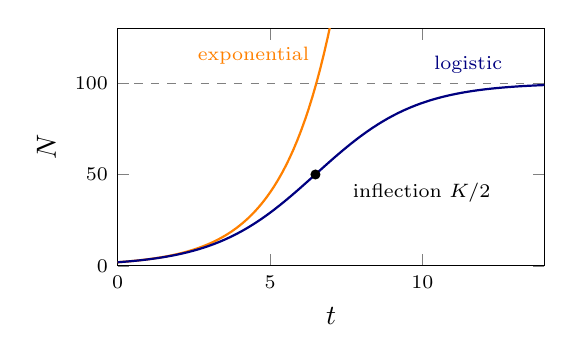
\begin{tikzpicture}
\begin{axis}[width=7cm,height=4.6cm,xlabel={$t$},ylabel={$N$},ymin=0,ymax=130,xmin=0,xmax=14,
  tick label style={font=\scriptsize}]
\addplot[domain=0:7.4,samples=60,thick,orange] {2*exp(0.6*x)};
\addplot[domain=0:14,samples=80,thick,NavyBlue] {100/(1+49*exp(-0.6*x))};
\addplot[dashed,gray] coordinates {(0,100)(14,100)};
\addplot[only marks,mark=*,mark size=1.6pt] coordinates {(6.49,50)};
\node[font=\scriptsize,anchor=west] at (axis cs:7.4,40) {inflection $K/2$};
\node[font=\scriptsize,orange,anchor=east] at (axis cs:6.6,115) {exponential};
\node[font=\scriptsize,NavyBlue] at (axis cs:11.5,110) {logistic};
\end{axis}
\end{tikzpicture}\hspace{4mm}
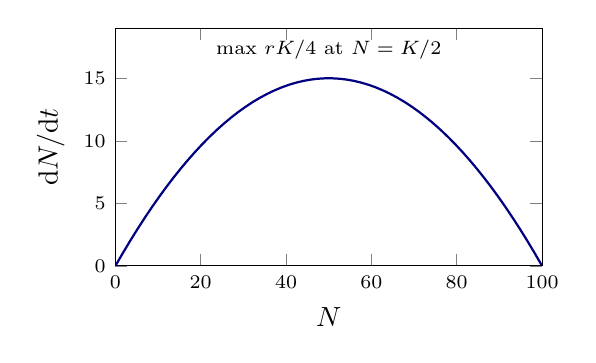
\begin{tikzpicture}
\begin{axis}[width=7cm,height=4.6cm,xlabel={$N$},ylabel={$\dd N/\dd t$},ymin=0,ymax=19,xmin=0,xmax=100,
  tick label style={font=\scriptsize}]
\addplot[domain=0:100,samples=60,thick,NavyBlue] {0.6*x*(1-x/100)};
\node[font=\scriptsize] at (axis cs:50,17.3) {max $rK/4$ at $N=K/2$};
\end{axis}
\end{tikzpicture}
\end{center}

Properties: $N\to K$; the growth rate is a parabola in $N$, largest ($rK/4$) at $N=K/2$, where the curve inflects; fixed
points $0$ (unstable, slope $+r$) and $K$ (stable, slope $-r$); near $K$ deviations decay as $e^{-rt}$, a
\textbf{relaxation time $1/r$}. $K$ is not a number written in the habitat: it is where the realised rate hits zero,
and it moves with food, space or climate.

\textbf{Four ways to write ``rate falls linearly with $N$''} (slide 20), depending on which realised rate is set to
$r(1-N/K)$:
\begin{center}\small
\begin{tabular}{ll}
\toprule
realised rate & model\\\midrule
$\frac1N\frac{\dd N}{\dd t}$ & continuous logistic $\dot N=rN(1-N/K)$\\
$(N_{t+1}-N_t)/N_t$ & discrete logistic $N_{t+1}=N_t[1+r(1-N_t/K)]$\\
$N_{t+1}/N_t$ & ``alternative'' $N_{t+1}=rN_t(1-N_t/K)$ (fixed point $K(1-1/r)$)\\
$\ln(N_{t+1}/N_t)$ & Ricker $N_{t+1}=N_te^{r(1-N_t/K)}$\\\bottomrule
\end{tabular}
\end{center}
Only the continuous one always approaches $K$ smoothly. The data checks (US census, rotifer culture) fit an S-curve
roughly, but slide 23 warns that the realised rate is often \emph{not} linear in $N$: the first few individuals
matter most.

\begin{chain}[: why discrete models can cycle and continuous one-variable models cannot]
A one-variable ODE moves along a line; to oscillate it would have to pass back through a point with the opposite
velocity, which a single-valued $\dot N=f(N)$ forbids. In a discrete map, births come in a pulse once per step, so the
population can \emph{jump over} $K$. A delay acts the same way: in the delayed logistic
$\dot N=rN(t)[1-N(t-\tau)/K]$ the brake responds to an old density, and cycles appear once $r\tau>\pi/2$.
\end{chain}

\subsection{The Ricker model: from stability to chaos}
\[
n_{t+1}=g(n_t)=n_t\exp\!\Bigl[r\Bigl(1-\frac{n_t}{K}\Bigr)\Bigr],\qquad g'(K)=1-r.
\]
$r$ ``determines the qualitative nature of the dynamics''; $K$ is where $n_{t+1}=n_t$ and only rescales ($n=Kx$
removes it).

\begin{chain}[: from the slope at $K$ to the whole route]
\begin{enumerate}
\item For a map, a fixed point is stable iff $|g'(n^*)|<1$: the deviation is multiplied by $g'$ each step.
\item $g'(K)=1-r$. For $0<r<1$ the multiplier is positive: monotone approach. For $1<r<2$ it is negative with
modulus $<1$: the population overshoots each step but by less each time (damped oscillation).
\item At $r=2$ the multiplier passes $-1$: overshoots stop shrinking, and a \textbf{2-cycle} is born.
\item The same thing happens to the 2-cycle (at $r=2.5265$, giving a 4-cycle), then the 4-cycle ($2.6564$, an
8-cycle)\dots: a \textbf{period-doubling cascade} accumulating at $r_\infty\approx2.6924$.
\item Beyond it the dynamics can be \textbf{chaotic}, interspersed with \textbf{periodic windows}.
\end{enumerate}
Biological meaning: \textbf{overcompensation}. At large $r$ a population just below $K$ grows so much it lands
further above $K$ than it was below; each correction is bigger than the error.
\end{chain}

\begin{trap}
Slide 25 labels its $r=2.5$ panel a ``4-point limit cycle''. The Ricker map at $r=2.5$ has period 2 (the 4-cycle lives
in $2.5265<r<2.6564$); a true 4-cycle example is $r=2.6$. If asked, say which value you use.
\end{trap}

\textbf{Bifurcation diagram}: for each $r$, plot the values visited in the long run; the number of points at a given
$r$ is the period. Zooming into it shows smaller copies of the whole (\textbf{fractal}: self-similarity at multiple
scales; slide 26 uses the logistic map's diagram and notes the principle is the same). The ratio of successive gaps
tends to Feigenbaum's constant $4.669$, the same for many one-hump maps (background).

\subsubsection*{Chaos}
\textbf{Deterministic chaos}: bounded, aperiodic behaviour with \textbf{sensitive dependence on initial conditions}.
Nearby starts separate as $\delta_t\approx\delta_0e^{\Lambda t}$ (Lyapunov exponent $\Lambda>0$; Ricker $r=3$:
$\Lambda\approx0.39$). The forecast horizon is $t\approx\ln(\text{range}/\delta_0)/\Lambda$: it grows only
\emph{logarithmically} with measurement precision (a 1000-fold better measurement buys $\ln 1000/0.39\approx18$
generations).

\begin{trap}
Chaos is \emph{not} randomness: no noise enters, and with exact initial values the series is reproducible; what fails
is prediction from imprecise data. Chaos is \emph{not} explosion: the orbit is bounded. And $r>2.69$ does not
guarantee chaos (periodic windows, e.g.\ $r=3.6$). A limit cycle repeats exactly; chaos never repeats.
\end{trap}

\subsection{The real world: Hassell's puzzle and its two resolutions}
\[
N_{t+1}=\lambda N_t(1+aN_t)^{-\beta},\qquad N^*=\frac{\lambda^{1/\beta}-1}{a},\qquad f'(N^*)=1-\beta\bigl(1-\lambda^{-1/\beta}\bigr).
\]
$\beta$ measures how abrupt density dependence is: $\beta\le1$ is \textbf{contest} competition (more parents never mean
fewer offspring; no hump, monotone approach for any $\lambda$); $\beta>1$ is \textbf{scramble} competition (a hump, so
overcompensation is possible). Instability needs both large $\beta$ and large $\lambda$.

Hassell, Lawton and May (1976) fitted $\lambda$ and $\beta$ to 24 insect populations: \textbf{22 of 24 showed monotonic
damping}, so ``natural populations exhibit relatively simple dynamics''. \textbf{The puzzle} (slide 30): simple models
allow chaos at high growth rates, insects have high growth rates, yet except for one or two cases no real population
has been shown to be chaotic, and near-universal simple behaviour ``does not make sense''.

\begin{chain}[: resolution 1, the lattice effect (Henson et al.\ 2001)]
\begin{enumerate}
\item Real organisms come in integers; the models use real numbers.
\item Integer counts with an upper bound give a \emph{finite} set of possible states.
\item A deterministic map on a finite set must eventually revisit a state (pigeonhole), and from then on repeats
exactly. So the integerised model is eventually periodic: \textbf{chaos gives way to limit cycles or extinctions}
(rounding a low point to 0).
\item The number of states grows with $K$, so cycles can be very long (Ricker, $K=10^4$: 82--155 generations). The
lattice effect excludes strict chaos, \textbf{not long-period cycles}, which in finite data look like chaos.
\end{enumerate}
\end{chain}

\begin{chain}[: resolution 2, model complexity (Turchin and Taylor 1992)]
\begin{enumerate}
\item Hassell et al.\ used a model with \textbf{one time lag and a simple functional form}.
\item Real density dependence is often \emph{delayed} (slow food plants, predators building up, cohorts maturing
later), which produces cycles.
\item A one-lag model fitted to such data sees only the average dependence of growth on current density, which slopes
gently down, and reports stability.
\item Fitting many models with more lags and flexible forms found the whole spectrum (damping, oscillatory damping,
limit cycles, chaos). Conclusion: ``use of overly simple models \ldots\ may be \textbf{biased in favour of finding
stability}.''
\end{enumerate}
Slide 35's analogy: a 4-D cube can cast a simple 2-D shadow. Complex high-dimensional objects can have simple
low-dimensional projections, so be careful inferring the object from the shadow.
\end{chain}

\begin{numbers}
Logistic: inflection $K/2$, max rate $rK/4$, relaxation $1/r$. Ricker thresholds: 2 (2-cycle), 2.5265 (4), 2.6564 (8),
2.6924 (chaos). Logistic map: $a=3, 3.449, 3.544,\dots\to3.570$. Hassell: 22/24 monotone. Turchin--Taylor: 14 insect +
22 vertebrate series. Doubling time $\ln 2/r$; human pop.\ doubling in 50\,yr $\Rightarrow r=0.0139$/yr.
\end{numbers}

\begin{statements}
\begin{enumerate}[label=\arabic*.]
\item ``In the Ricker model, raising $K$ can turn a stable population chaotic.''
\F Only $r$ sets the type of dynamics; $K$ rescales.
\item ``The continuous logistic can show damped oscillations if $r$ is large enough.''
\F A one-dimensional ODE cannot oscillate; it approaches $K$ monotonically for any $r>0$. Oscillation needs discrete
steps or delays.
\item ``A population growing logistically adds individuals fastest when it is smallest, because its per-capita rate is highest then.''
\F The per-capita rate is highest at small $N$, but the total rate $rN(1-N/K)$ peaks at $K/2$.
\item ``Chaos and a long limit cycle can both look irregular, but only the cycle repeats exactly.''
\T That is exactly why the lattice effect rules out strict chaos but not long cycles.
\item ``If a chaotic system is deterministic, a better measurement of the initial state will always extend the forecast horizon in proportion.''
\F The horizon grows only with the \emph{logarithm} of precision.
\item ``Hassell et al.'s finding that 22 of 24 populations are monotone shows that chaos is rare in nature.''
\F It shows that a one-lag, simple-form model fitted to the data says so; Turchin and Taylor showed such models are biased toward stability.
\item ``The lattice effect explains why deterministic chaos is not seen, because integer populations with an upper bound have finitely many states.''
\T That is the argument of slide 33 (it says nothing against long cycles).
\item ``The exponential model is useless because no population grows exponentially for long.''
\F It is the null model (``first law''); departures from it are what the subject studies.
\end{enumerate}
\end{statements}

\begin{longans}[: ``Simple models predict chaos at high growth rates, yet chaos is almost never observed. Discuss.'']
(1) Ricker/logistic map: stability for $0<r<2$, period doubling, chaos beyond 2.69; define chaos (deterministic,
bounded, aperiodic, SDIC). (2) Expectation: insects have high $\lambda$, so chaos should be common. (3) Hassell et al.\
1976: 22/24 monotone. (4) Resolution 1, lattice effect: integers + bound $\Rightarrow$ finite states $\Rightarrow$
eventual periodicity or extinction; long cycles still possible. (5) Resolution 2, model complexity: one lag and a
rigid form bias toward stability; Turchin and Taylor's flexible multi-lag fits found the full spectrum including
chaos. (6) Moral: the model is not the world; a low-dimensional projection can hide complex dynamics.
\end{longans}

% ===================================================================
\section{Competition and invasions (EE04)}
% ===================================================================

\subsection{What competition is}
\textbf{Competition}: any use or defence of a resource by one individual that reduces its availability to others.
\begin{itemize}
\item \textbf{Intraspecific}: within a species. The density-dependent fall of growth in EE03 ($r'=r(1-N/K)$) is
intraspecific competition; so is competition for mates.
\item \textbf{Interspecific}: two species competing for the same \emph{limiting} resource. Two defining features: it is
\textbf{non-trophic} (neither eats the other), and it \textbf{reduces the growth rate or equilibrium number of at
least one} of them. If the species do not affect each other, there is no competition.
\end{itemize}
Exploitation (using the resource up) and interference (blocking access) are both competition; the models here are
about exploitation. Competing is not fighting: two shops on a street compete for a limited pool of customers whether
or not the owners ever meet.

\subsection{Competitive exclusion and the $R^*$ rule}
\textbf{Gause}: \emph{Paramecium aurelia} and \emph{P.\ caudatum} each reach a carrying capacity alone; together,
\emph{P.\ aurelia} keeps increasing and \emph{P.\ caudatum} declines. \textbf{Competitive exclusion principle}: ``no
two species with the same niche can coexist''. \textbf{Tilman (1981)}: diatoms competing for silicate; ``two species
cannot coexist on a single limiting resource''. (Slide 8 notes the original figure's legend should be inverted; do
not quote the winner from the colours.)

\begin{chain}[: why the lowest $R^*$ wins]
\begin{enumerate}
\item Species $i$ grows at per-capita rate $f_i(R)-m_i$, where $f_i$ rises with resource level $R$ and $m_i$ is its
loss rate. It can grow only while $R>R^*_i$, the break-even level where $f_i(R^*_i)=m_i$.
\item Alone, each species draws $R$ down to its own $R^*$ and stops there.
\item Together, with $R^*_1<R^*_2$: species 1 keeps pushing $R$ down towards $R^*_1$. At any $R<R^*_2$ species 2's
growth is negative \emph{even though it is still eating}. So species 2 cannot persist.
\item Therefore the winner is the species that can maintain positive growth at the lowest resource level, not the one
that grows fastest when food is plentiful. With a Monod response $f=\mu R/(k+R)$: $R^*=mk/(\mu-m)$.
\end{enumerate}
\end{chain}

\begin{worked}[: the fast grower loses]
$m=0.2$. A: $\mu=0.8$, $k=2$, $R^*_A=0.667$. B: $\mu=0.6$, $k=1$, $R^*_B=0.5$. At $R=10$, A grows faster (0.667 vs
0.545). But B draws $R$ down to 0.5, where A's growth is $0.16<0.2$: A goes extinct. And adding food to help the loser
does not change either $R^*$, so it does not change the winner, only the winner's numbers.
\end{worked}

\subsection{The Lotka--Volterra competition model}
\[
\frac{\dd N_1}{\dd t}=\frac{r_1N_1(K_1-N_1-\alpha_{12}N_2)}{K_1},\qquad
\frac{\dd N_2}{\dd t}=\frac{r_2N_2(K_2-N_2-\alpha_{21}N_1)}{K_2}.
\]
$\alpha_{12}$ is the effect of one individual of species \textbf{2 on species 1}, measured in \emph{intraspecific
equivalents}: $\alpha_{12}=3$ means one individual of species 2 suppresses species 1 as much as three of its own;
$\alpha_{12}=0$, no effect; $\alpha_{12}=1$, ecological equivalents.

\textbf{Isoclines} (zero growth): species 1: $N_1=K_1-\alpha_{12}N_2$ (intercepts $K_1$ on the $N_1$ axis,
$K_1/\alpha_{12}$ on the $N_2$ axis); species 2: $N_2=K_2-\alpha_{21}N_1$ (intercepts $K_2$ and $K_2/\alpha_{21}$). Species 1
grows when $N_1+\alpha_{12}N_2<K_1$: the crowding it feels (own numbers plus competitors in its own units) is below what
it tolerates. So each species increases below (inside) its isocline and decreases above it.

\begin{center}
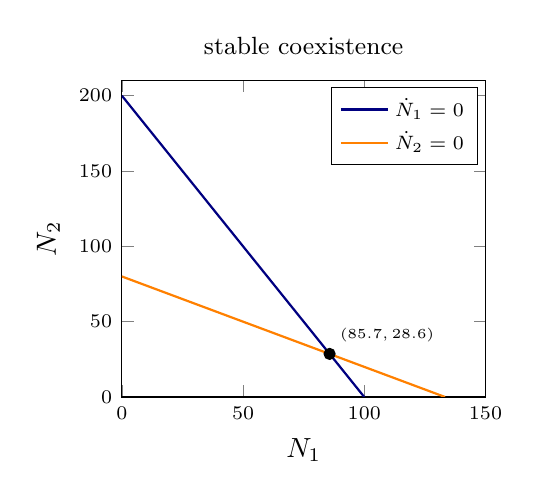
\begin{tikzpicture}
\begin{axis}[width=6.2cm,height=5.6cm,xlabel={$N_1$},ylabel={$N_2$},xmin=0,xmax=150,ymin=0,ymax=210,
  title={\small stable coexistence},tick label style={font=\scriptsize},
  legend style={font=\scriptsize,at={(0.98,0.98)},anchor=north east}]
\addplot[thick,NavyBlue] coordinates {(100,0)(0,200)}; \addlegendentry{$\dot N_1=0$}
\addplot[thick,orange] coordinates {(0,80)(133.3,0)}; \addlegendentry{$\dot N_2=0$}
\addplot[only marks,mark=*] coordinates {(85.7,28.6)};
\node[font=\tiny,anchor=south west] at (axis cs:86,30) {$(85.7,28.6)$};
\end{axis}
\end{tikzpicture}\hspace{3mm}
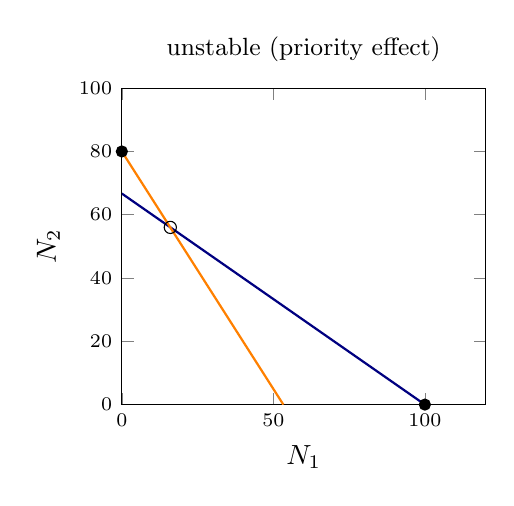
\begin{tikzpicture}
\begin{axis}[width=6.2cm,height=5.6cm,xlabel={$N_1$},ylabel={$N_2$},xmin=0,xmax=120,ymin=0,ymax=100,
  title={\small unstable (priority effect)},tick label style={font=\scriptsize}]
\addplot[thick,NavyBlue] coordinates {(100,0)(0,66.7)};
\addplot[thick,orange] coordinates {(0,80)(53.3,0)};
\addplot[only marks,mark=o,mark size=2.2pt] coordinates {(16,56)};
\addplot[only marks,mark=*] coordinates {(100,0)(0,80)};
\end{axis}
\end{tikzpicture}

\small $K_1=100$, $K_2=80$. Left: $\alpha_{12}=0.5$, $\alpha_{21}=0.6$. Right: $\alpha_{12}=\alpha_{21}=1.5$; filled dots stable,
open dot a saddle.
\end{center}

\begin{chain}[: the four outcomes as two invasion tests]
Ask: can a species increase when \emph{rare}, with the other sitting at its own $K$?
\begin{itemize}
\item Can 2 invade 1? Rare species 2 feels crowding $\alpha_{21}K_1$, so it grows iff $\alpha_{21}K_1<K_2$, i.e.\ $K_1<K_2/\alpha_{21}$.
\item Can 1 invade 2? Iff $\alpha_{12}K_2<K_1$, i.e.\ $K_2<K_1/\alpha_{12}$.
\end{itemize}
\begin{center}\small
\begin{tabular}{lll}
\toprule
1 invades 2? & 2 invades 1? & outcome\\\midrule
yes & no & species 1 wins\\
no & yes & species 2 wins\\
yes & yes & \textbf{stable coexistence} (whoever becomes rare grows back)\\
no & no & \textbf{unstable equilibrium}: priority effect, the start decides\\\bottomrule
\end{tabular}
\end{center}
Coexistence therefore requires $\alpha_{12}<K_1/K_2$ \emph{and} $\alpha_{21}<K_2/K_1$: \textbf{each species limits itself
more than it limits the other}. Slide 12: in 3 of the 4 cases one species drives the other extinct.
\end{chain}

At a coexistence point, $N_1^*=\dfrac{K_1-\alpha_{12}K_2}{1-\alpha_{12}\alpha_{21}}$,
$N_2^*=\dfrac{K_2-\alpha_{21}K_1}{1-\alpha_{12}\alpha_{21}}$, each below its own $K$. The Jacobian determinant is
proportional to $1-\alpha_{12}\alpha_{21}$, so an interior point that \emph{exists} is stable iff $\alpha_{12}\alpha_{21}<1$.

\begin{trap}
\begin{itemize}
\item Index order: $\alpha_{12}$ is the effect of 2 \emph{on} 1. Swapping it swaps the isoclines.
\item $\alpha_{12}\alpha_{21}<1$ is necessary, not sufficient: with unequal $K$ the interior point may not exist
(e.g.\ $\alpha_{21}K_1>K_2$ gives $N_2^*<0$). Check both invasion conditions.
\item $\alpha>1$ does not by itself mean exclusion, if $K_1/K_2$ is large enough.
\item ``3 of 4 outcomes are exclusion'' is a statement about the model's regions, not a claim that exclusion is common in
nature.
\end{itemize}
\end{trap}

\begin{worked}[: 2025 mid-sem Q11]
$K_1=250$, $\alpha_{12}=1.4$; $K_2=1500$, $\alpha_{21}=0.9$. Species 1's isocline runs $(250,0)$--$(0,178.6)$; species 2's
runs $(1667,0)$--$(0,1500)$. Species 2's line lies outside species 1's on both axes, so \textbf{species 2 wins} from any
start, ending at $(0,1500)$. ($r$ values do not affect the outcome, only the speed.)
\end{worked}

\subsection{Invasive species: super-competitors}
An invader arriving without its natural enemies and with efficient resource use acts like a species with large
$\alpha_{\text{inv}\to\text{nat}}$ and small $\alpha_{\text{nat}\to\text{inv}}$: the ``invader wins'' region.
\textbf{Kerala}: the 2018--2019 floods released aquaculture and aquarium fish (arapaima, up to 200\,kg; alligator gar, up to
137\,kg). A 2021 survey of 44 rivers and 53 reservoirs found \textbf{28 alien fish and 4 alien aquatic weeds, 7
established}; main routes: aquarium trade and aquaculture. Water hyacinth (also in the Mula river at Dapodi, per the
wrap-up lecture) is turned into crafts and sarees in Kerala, Assam and West Bengal. Self-study: Asian carps,
\emph{Caulerpa taxifolia}.

Competition is only one mechanism of invasion success: propagule pressure, disturbance, and demographic and genetic
accidents of small founding groups (bottlenecks, inbreeding) also matter; that is why most introductions fail
(background: Sakai et al.\ 2001).

\subsection{Why similar species coexist: the niche and its partitioning}
The \textbf{niche} is an $n$-dimensional hypervolume of conditions and resources. Two meanings:
\begin{itemize}
\item \textbf{Population-persistence niche} (Hutchinson): the range of conditions that allow a population to persist
(positive growth rate) in a place: \emph{where it can live}.
\item \textbf{Resource-utilisation niche} (MacArthur, Levins): what members of the population actually do, in particular
how they use resources: \emph{what it does}.
\end{itemize}
\textbf{Fundamental} niche: where a species could persist without enemies and competitors; \textbf{realised} niche:
where it actually does. Partitioning lowers overlap and so lowers $\alpha$ until the coexistence conditions hold: it
changes the parameters, not the model.

\begin{center}\small
\begin{tabularx}{\textwidth}{lX}
\toprule
type & case and logic\\\midrule
spatial & Gause: \emph{P.\ caudatum} feeds in the top layer, \emph{P.\ bursaria} at the bottom; they coexist.\\
spatial & Connell's barnacles: \emph{Chthamalus} high on the shore (\emph{Balanus} desiccates there); \emph{Balanus} in the
middle, where it outcompetes \emph{Chthamalus} for space; lower, \emph{Balanus} suffers predation. Physical limits set
the upper edge of one species, competition the lower edge of the other: realised $<$ fundamental.\\
temporal & Spiny mice in Israel: common (\emph{Acomys cahirinus}) nocturnal, golden (\emph{A.\ russatus}) diurnal. Remove the
common species and the golden one becomes nocturnal: the separation is \emph{induced} by competition.\\
morphological & Character displacement: traits of related species differ \emph{more where they co-occur} than where
they are apart (beak depths of Galápagos ground finches on different islands).\\
conditional & Park's \emph{Tribolium}: \emph{confusum} wins cool-dry (100\,\%), \emph{castaneum} wins warm-moist (100\,\%).\\\bottomrule
\end{tabularx}
\end{center}

\begin{keyidea}[: Park's lesson]
A higher single-species equilibrium does \emph{not} guarantee victory. Cool-moist: \emph{castaneum} is larger alone
(45.2 vs 28.2) yet loses 71\,\% of contests; warm-moist: \emph{confusum} is larger (41.2 vs 38.3) and loses every
contest. $K$ is half the story; the competition coefficients, which change with temperature and humidity, decide the
contest. If conditions switch faster than exclusion takes, neither wins permanently.
\end{keyidea}

\begin{statements}
\begin{enumerate}[label=\arabic*.]
\item ``A lion eating a zebra is an extreme form of interspecific competition.''
\F Competition is non-trophic; eating is predation.
\item ``The species with the highest growth rate at high resource density wins exploitative competition.''
\F The species with the lowest $R^*$ wins; the fast grower at high food can lose.
\item ``If $\alpha_{12}\alpha_{21}<1$, the two species must coexist.''
\F Necessary for a stable interior point but not sufficient; with unequal $K$, check $\alpha_{12}<K_1/K_2$ and $\alpha_{21}<K_2/K_1$.
\item ``In the unstable-equilibrium case, the winner is decided by the starting numbers.''
\T Neither can invade the other; the saddle's separatrix splits the plane (priority effect, a kind of bistability).
\item ``The golden spiny mouse is diurnal because diurnality is in its fundamental niche only.''
\F It becomes nocturnal when the competitor is removed: diurnality is its \emph{realised} niche, induced by competition.
\item ``Character displacement predicts that two related species are \emph{more} similar where they co-occur.''
\F More \emph{different} where they co-occur.
\item ``Coexisting competitors probably partition the niche, though showing how is often hard.''
\T This is the wrap-up lecture's own summary for competition.
\item ``Feeding an endangered native fish more will help it against an invader limited by the same single food.''
\F Feeding raises supply but leaves both $R^*$ unchanged; the invader still draws food down below the native's break-even.
\end{enumerate}
\end{statements}

\begin{longans}[: ``In 3 of 4 cases L--V competition predicts exclusion, yet many similar species coexist. Resolve.'']
(1) Model, isoclines, the four outcomes via invasion tests; coexistence iff each limits itself more than the other.
(2) Exclusion seen in simple lab settings: Gause (\emph{aurelia} vs \emph{caudatum}), Tilman (one resource), $R^*$.
(3) Mechanism 1, niche partitioning lowers $\alpha$: spatial (\emph{caudatum}/\emph{bursaria}; barnacles), temporal
(spiny mice removal), morphological (character displacement). (4) Mechanism 2, conditional outcomes and fluctuating
environments: Park's \emph{Tribolium}. (5) The model gives a precise question; experiments find which condition holds.
\end{longans}

% ===================================================================
\section{Predation (EE05)}
% ===================================================================

\subsection{Definition and types}
\textbf{Predation}: the process by which an organism eats all or part of another organism. Reasons to study it:
economic (pests, harvests), ecological (community organisation, conservation), evolutionary (it shapes the traits of
both sides). Types:
\begin{itemize}
\item \textbf{herbivory}: animals eat plants, often partially;
\item \textbf{carnivory}: an animal \emph{or plant} eats animals (a pitcher plant counts);
\item \textbf{parasitoidism}: eggs laid on or near a host that the offspring later kill;
\item \textbf{parasitism}: living on or in a host and feeding from it without (usually) killing it;
\item \textbf{cannibalism}: predator and prey of the same species.
\end{itemize}
Unlike competition, which divides a supply, predation \emph{transfers} biomass and kills the loser, so predator and
prey numbers feed back on each other: more prey feed more predators, more predators remove more prey.

\subsection{The hare--lynx cycle: intrinsic or extrinsic?}
Hudson's Bay Company fur returns (Elton 1924), $\sim$1850--1930: snowshoe hare and lynx cycle with a period of about
10 years, the lynx following the hare. Are the cycles \textbf{intrinsic} (generated by the interacting populations:
food, predators, disease) or \textbf{extrinsic} (weather, sunspots)?

Background (Molles): the sunspot hypothesis failed (the cycles do not match); ``overpopulation'' hypotheses
(disease, stress, starvation) and ``predators drive it'' were each insufficient alone. \textbf{Krebs et al.\ (1995)},
8 years, 1-km$^2$ blocks: excluding predators doubled hare density, adding food tripled it, both together raised it
\textbf{eleven-fold}.

\begin{chain}[: what $\times2$, $\times3$, $\times11$ means]
If the two factors acted independently and additively, the joint effect would be $1+1+2=4$; independently and
multiplicatively, $2\times3=6$. The observed 11 exceeds both: the factors \textbf{interact synergistically}. A
well-fed population converts lower predation into growth, and a predator-free one converts extra food into
numbers. So no single-factor hypothesis can work: the cycle is an interaction of \textbf{three trophic levels}
(plants, hares, predators).
\end{chain}

\subsection{The Lotka--Volterra predator--prey model}
\[
\frac{\dd H}{\dd t}=rH-pHP,\qquad \frac{\dd P}{\dd t}=apHP-mP,\qquad
H^*=\frac{m}{ap},\quad P^*=\frac rp .
\]
Prey grow exponentially and are removed in proportion to encounters $HP$ (capture coefficient $p$); predators die at
rate $m$ without prey and convert captured prey into offspring with efficiency $a$.

\begin{chain}[: reading the equilibrium]
\begin{enumerate}
\item The \emph{prey} stop changing when predators are at $P^*=r/p$: just enough to eat the prey's growth.
\item The \emph{predators} stop changing when prey are at $H^*=m/(ap)$: just enough to feed them.
\item So the prey level is set by the \emph{predator's} traits ($m$, $a$, $p$), and the predator level by the
\emph{prey's} growth rate $r$. Doubling $r$ doubles the predators and leaves prey unchanged.
\end{enumerate}
\end{chain}

\begin{chain}[: why the predator lags]
Predators increase whenever $H>H^*$, so they keep increasing while prey are abundant, and peak only when the
declining prey fall back through $H^*$. Prey increase whenever $P<P^*$, so their rise is timed by the predators' crash.
Each species' turning points are set by the \emph{other} crossing its isocline: prey peak first, predators a quarter
cycle later (for small cycles).
\end{chain}

\textbf{Neutral cycles.} Linearising gives eigenvalues $\pm i\sqrt{rm}$ (small-cycle period $2\pi/\sqrt{rm}$), and the
quantity $V=apH-m\ln H+pP-r\ln P$ is conserved along every solution, so each orbit is a closed curve. The model
``only admits oscillatory behaviour''.

\textbf{Assumptions} (slide 7): (1) prey growth limited only by predation; (2) a specialist predator that needs this
prey; (3) a constant environment; (4) random encounters in a homogeneous environment.

\begin{trap}
The L--V cycles are \textbf{neutral and structurally unstable}. A shock moves the system to another orbit, where it
stays (no preferred amplitude), and any small extra term in the equations turns the closed orbits into spirals.
Real systems always have such terms, so the model's perfect cycles cannot be the explanation of real cycles.
\end{trap}

\textbf{Volterra's principle} (background): killing prey and predators at the same extra rate $\delta$ gives
$r\to r-\delta$, $m\to m+\delta$, so $H^*$ \emph{rises} and $P^*$ \emph{falls}. A broad pesticide that also kills natural
enemies can make a pest more abundant.

\subsection{Density-dependent prey, and the puzzle}
With logistic prey, $\dot H=rH(1-H/K)-pHP$: the predator isocline is still $H^*=m/(ap)$, the prey isocline slopes down,
$P=(r/p)(1-H/K)$, and $P^*=(r/p)(1-H^*/K)$, positive only if $K>m/(ap)$ (otherwise predators cannot be fed and die out).
The Jacobian now has negative trace ($-rH^*/K$) and positive determinant: a \textbf{stable equilibrium}, usually a
spiral. Prey self-limitation acts like friction on an oscillator.

\begin{keyidea}[: the three-part puzzle (slide 9)]
(1) Real data show cycles. (2) The highly unrealistic L--V model shows cycles. (3) Realistic (density-dependent)
L--V models do \emph{not}. The simple model gets the observation for the wrong reason, and adding realism loses it.
``Enter lab experiments.''
\end{keyidea}

(Background: the answer depends on which realism is added. Prey self-limitation damps cycles; a \emph{saturating}
predator (Holling type II, $g=aH/(1+ahH)$, maximum $1/h$) destabilises, because a satiated predator removes a
smaller fraction of prey as prey increase. Together they give stable limit cycles of fixed amplitude once $K$ is large:
the ``paradox of enrichment''.)

\subsection{Laboratory tests: Gause and Huffaker}
\begin{center}\small
\begin{tabularx}{\textwidth}{lX}
\toprule
Gause (\emph{Paramecium} prey, \emph{Didinium} predator) & result\\\midrule
(a) simple culture, no refuge & predator eats all prey, then starves: \textbf{both extinct}\\
(b) sediment refuge for prey & predator eats exposed prey, then starves: \textbf{predator extinct}, prey recover\\
(c) one prey + one predator added every third day & \textbf{sustained oscillations}\\\bottomrule
\end{tabularx}
\end{center}
Gause's conclusion: the system would be driven to extinction if left to itself; oscillations are possible only with
constant interference from outside.

\textbf{Huffaker}: ``Gause's system was too simple and lacked environmental heterogeneity.'' Prey mite
\emph{Eotetranychus} on oranges, predatory mite \emph{Typhlodromus}; petroleum-jelly barriers; prey disperse by
ballooning on silk, predators must crawl; only $\sim$5\,\% of each orange exposed. Simple layouts failed; the most
elaborate, \textbf{120 oranges}, gave \textbf{three oscillations over about six months}.

\begin{chain}[: why patchiness rescues the system]
Within one patch the efficient predator wins and the prey die out locally. But prey disperse faster than
predators, so they reach empty patches before predators find them. The whole system persists as local extinctions
balanced by recolonisations: a \textbf{metapopulation}. In Levins' model the occupied fraction is $p^*=1-e/c$, positive
only if colonisation $c$ exceeds extinction $e$. Hence ``if the predator is efficient, the prey can survive only in a
patchy environment''. This breaks L--V assumption (4), random encounter in a homogeneous space. Gause's immigration
in (c) does the same job as Huffaker's dispersal: rescue from outside the local system.
\end{chain}

\textbf{In nature} (slide 15): a very complicated story; all kinds of dynamics are seen, because of multiple prey and
predators, spatial heterogeneity and refugia, predator efficiency changing over time, and evolution of both sides.
Wrap-up lecture: in simple homogeneous systems prey are driven extinct; real systems are heterogeneous and both sides
evolve strategies, giving a dynamic, ever-shifting equilibrium.

\subsection{Anti-predator strategies}
\begin{center}\small
\begin{tabularx}{\textwidth}{lXl}
\toprule
strategy & logic & example\\\midrule
aposematism & conspicuous signal advertising danger or distaste & yellow-winged darter\\
crypsis & resemble the background or an object & dead-leaf mantis, tawny frogmouth\\
Batesian mimicry & harmless mimic copies a defended model's signal & drone fly / honey bee\\
Müllerian mimicry & several defended species share one signal & \emph{Heliconius}\\
catalepsis & play dead & opossum\\
intimidation display & startle or bluff & eyespot moths\\
group living & vigilance, dilution, mobbing, confusion, alarm calls/pheromones & mobbing birds, aphids\\
chemical defence & toxic, smelly, distasteful & skunk, bombardier beetle\\\bottomrule
\end{tabularx}
\end{center}

\begin{chain}[: why toxins come with warning colours]
A poisoned predator does not save the prey it has already killed. The benefit of toxicity reaches the prey
\emph{population} only if predators \emph{learn} to avoid the species after a sample. Learning needs a memorable,
recognisable signal. So distastefulness and conspicuous colour evolve together.
\end{chain}

\begin{chain}[: why a Batesian mimic must be rarer than its model]
A predator attacking a signal-bearer gains $G$ from a mimic and pays $C$ for a model. If a fraction $q$ are models, the
expected gain is $(1-q)G-qC$; it attacks only if $q<G/(G+C)$. As mimics become common, the signal loses its
information and predators start attacking: the mimic is protected only while rarer than the model. In Müllerian
mimicry every bearer is defended, so each added species only \emph{shares} the cost of educating predators.
\end{chain}

\begin{numbers}
Hare--lynx period $\approx$10\,yr. Krebs: predators out $\times2$, food $\times3$, both $\times11$. L--V: $H^*=m/(ap)$,
$P^*=r/p$, period $2\pi/\sqrt{rm}$. Huffaker: 120 oranges, 3 oscillations, $\sim$6 months, 5\,\% of each orange exposed.
\end{numbers}

\begin{statements}
\begin{enumerate}[label=\arabic*.]
\item ``In the L--V model, increasing the prey's growth rate increases the equilibrium prey density.''
\F $H^*=m/(ap)$ does not involve $r$; predators ($P^*=r/p$) absorb the extra growth.
\item ``The L--V cycles return to their original amplitude after a disturbance.''
\F They are neutral: a disturbance shifts the system to a new orbit. A cycle that returns is a \emph{limit cycle}.
\item ``Adding prey density dependence to L--V makes the cycles more realistic.''
\F It damps them to a stable point: that is part (3) of the puzzle.
\item ``In Gause's refuge experiment both species went extinct.''
\F Only the predator did; the hidden prey recovered.
\item ``Huffaker's result shows that spatial heterogeneity with differential dispersal can allow predator and prey to persist together.''
\T Prey escaped to new patches ahead of predators (metapopulation dynamics).
\item ``A toxin that kills the predator protects the individual prey that was eaten.''
\F The benefit works through predator learning, hence warning colours.
\item ``Müllerian mimics are parasites on each other's signal.''
\F All are defended; sharing the signal lowers each species' losses to predator education. Batesian mimics are the ``parasites''.
\item ``A prey trait that reduces detection by a predator shows predator--prey coevolution.''
\F Coevolution needs reciprocal change in \emph{both} parties; a one-sided adaptation is not evidence of it (2022 mid-sem Q3).
\item ``Food and predators each affect hare numbers independently.''
\F $11>2\times3$: they interact.
\end{enumerate}
\end{statements}

\begin{longans}[: ``Real predator--prey systems cycle, and so does the L--V model; yet we do not believe the model. Explain.'']
(1) Model, equilibrium, neutral closed orbits, predator lag; assumptions. (2) Structural instability: neutral orbits,
any extra term gives spirals; with logistic prey the cycles damp out. (3) The three-part puzzle. (4) Lab: Gause
(extinction unless immigration), Huffaker (patchiness and dispersal $\Rightarrow$ metapopulation persistence).
(5) Field: Krebs, three trophic levels interacting ($\times11$). (6) Nature: multiple species, heterogeneity, changing
efficiency, evolution of defences. Conclusion: cycles are real, but their cause is not the mechanism of the basic model.
\end{longans}

% ===================================================================
\section{Eutrophication and alternative stable states (EE06)}
% ===================================================================

\subsection{Lake types: boxes and a continuum}
\textbf{Classical} (Naumann, Thienemann): \textbf{oligotrophic} (low productivity, clear water), \textbf{eutrophic}
(high productivity, green water from phytoplankton), \textbf{dystrophic} (low conductivity, brown humic water), then
``extinction'' as the basin fills with sediment. Qualitative signs: oligotrophic lakes have an \emph{orthograde} summer
oxygen profile (oxygen stays high with depth), eutrophic lakes a \emph{clinograde} one (oxygen falls to zero in the
hypolimnion).

\textbf{Modern}: oligo- and eutrophic are regions of a \textbf{continuum}, separated by limits such as $P_{tot}$ during
spring circulation (µg\,L$^{-1}$): ultra-oligotrophic $<5$, oligotrophic 5--10, mesotrophic 10--30, eutrophic 30--100,
hypereutrophic $>100$. Since trophic state is a biological phenomenon, several criteria are needed.

\begin{trap}[: one number can misclassify]
Schöhsee (mean depth 13\,m, $P_{tot}\approx20$) is mesotrophic by phosphorus but has an anoxic hypolimnion
(``eutrophic'' traditionally). Lake Constance (mean depth $\sim$100\,m, $P_{tot}\approx100$ in 1980) is eutrophic by
phosphorus yet its bottom water stayed $\sim$50\,\% saturated. The difference is \textbf{morphometry}: a huge hypolimnion
holds enough oxygen from spring overturn to decompose sinking matter; a small one does not.
\end{trap}

\textbf{What sets trophic status} (slide 5): (1) basin shape (mean depth); (2) the drainage basin (erosion, soils);
(3) climate (precipitation, temperature); (4) human activity (\textbf{cultural eutrophication}: fertiliser, sewage,
industrial waste). Large deep lakes are less productive because (i) loading per unit volume is lower when the lake is
big relative to its watershed, (ii) little of the epilimnion touches the sediment, so few nutrients return to the lit
zone, and (iii) longer retention times let more phosphorus settle out. Background (OECD/Vollenweider):
$P_L=1.55[P_{in}/(1+\sqrt{\tau_w})]^{0.82}$.

\subsection{How a lake becomes eutrophic}
\begin{chain}[: the eutrophication chain, and why it self-accelerates]
\begin{enumerate}
\item \textbf{Nutrient enrichment}, chiefly phosphorus (sewage, P-detergents, fertiliser, erosion). P limits because it
is relatively immobile in soil, unlike N. Sewage has N:P $\approx$ 4:1, so heavy sewage can even shift a lake to
N limitation.
\item \textbf{More production}: algal blooms, including cyanobacteria (\emph{Anabaena}, \emph{Microcystis}): scums,
toxins, odours. Periphyton overgrows and shades submerged plants.
\item \textbf{Less light}; dead algae sink and decompose, consuming \textbf{oxygen in the hypolimnion}.
\item \textbf{Anoxic sediment releases phosphorus} (internal loading; background chemistry: Fe(III) phosphate is
reduced to soluble Fe(II) and phosphate).
\item More P $\Rightarrow$ more algae $\Rightarrow$ more anoxia $\Rightarrow$ more P: every link positive, so the loop is
\textbf{reinforcing}. Internal loading ``sets in motion the self-acceleration of eutrophication''.
\item pH rises (intense photosynthesis), turning ammonium into toxic ammonia; oxygen collapses: \textbf{fish kills}.
\end{enumerate}
Not only a small-lake problem: Caspian Sea (2003), Lake Erie. Anoxic hypolimnia exist only in stratified lakes, which is
why a deep lake with a big hypolimnion tolerates more phosphorus.
\end{chain}

\subsection{Reversal: Lake Washington and the lag}
Lake Washington (Seattle): sewage from treatment plants in the 1940s--50s; in 1955 \emph{Oscillatoria rubescens}
appears (Edmondson's alarm); early 1960s transparency $\sim$1\,m (``Lake Stinko''); sewage diversion to Puget Sound
complete \textbf{1968}; phosphorus falls within $\sim$2 years; transparency 3--4\,m (1970--75); \textbf{1976}: large
\emph{Daphnia} return and transparency doubles to $\sim$10\,m. (Slide 11's ``sewage $\to$ oligotrophy $\to$ Lake
Stinko'' is a slip: sewage made it eutrophic.) Lake Constance went from 6 to 87 to 8\,µg\,L$^{-1}$ with tertiary
treatment and P-free detergents.

\begin{chain}[: why the second jump was not phosphorus]
Phosphorus had already fallen by 1970, giving 3--4\,m. The jump to 10\,m came with the return of large \emph{Daphnia},
which graze phytoplankton. They returned because filamentous cyanobacteria that clog their filters disappeared
(bottom-up) and mysid shrimp predation fell (top-down). So food-web structure, not just nutrients, decides how far a
lake recovers.
\end{chain}

\textbf{Why recovery lags} after loading is cut: (i) the water must be exchanged; (ii) phosphorus stored in sediments keeps
being released, even faster as the water concentration falls; (iii) at peak eutrophication algae were limited by N or
light, so P must fall a long way before it limits; (iv) long-lived planktivorous fish keep suppressing grazers.

\subsection{Not so simple: alternative stable states}
\textbf{Lake Veluwe} (Netherlands): as phosphorus rose, charophyte vegetation collapsed abruptly (late 1960s--70s); when
loading was cut, the vegetation returned only in the 1990s, at a \textbf{much lower} phosphorus level.
\textbf{Hysteresis}: the path back differs from the path out.

\begin{chain}[: why a shallow lake has two stable states]
\begin{enumerate}
\item Sign rule (slide 16): multiply the signs round a loop. Turbidity $\to$ light on the bed ($-$) $\to$ vegetation
($+$) $\to$ sediment resuspension ($-$) $\to$ turbidity ($+$): $(-)(+)(-)(+)=+$. The direct pair vegetation
$\dashv$ turbidity $\dashv$ vegetation gives $(-)(-)=+$ too. The loop is \textbf{reinforcing}.
\item A reinforcing loop alone means runaway. But it saturates at both ends: plant cover cannot exceed the bed, and
clear water has no more turbidity to remove; once plants are gone, the plant part of the loop has nothing left to act on.
\item Reinforcing loop + saturation at both ends = \textbf{two self-stabilising states}: clear and vegetated, or turbid
and unvegetated. A small disturbance from either is pushed back by the same loop.
\item Plants keep water clear by taking up nutrients, sheltering \emph{Daphnia} from fish, and stopping resuspension.
Fish keep it turbid by eating \emph{Daphnia} and stirring sediment.
\item In \emph{deep} lakes light reaches the bed only near the shore, so plants cannot cover most of the lake and the loop is
too weak: deep lakes respond smoothly (background).
\end{enumerate}
\end{chain}

\textbf{Graphical model} (slide 17), three assumptions: turbidity rises with nutrients; vegetation lowers turbidity;
vegetation vanishes above a critical turbidity. Result: at low nutrients only the clear state exists, at high nutrients
only the turbid state, and in between \textbf{both}, separated by an unstable equilibrium. Crossing the edge of the
overlap gives a \textbf{catastrophic regime shift} (tipping point). Making the model more realistic does not change
this qualitative conclusion.

\begin{center}
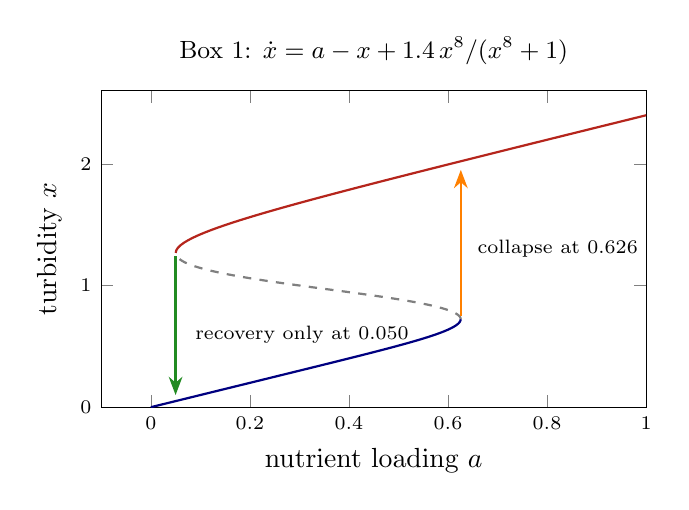
\begin{tikzpicture}
\begin{axis}[width=8.5cm,height=5.6cm,xlabel={nutrient loading $a$},ylabel={turbidity $x$},
  xmin=-0.1,xmax=1.0,ymin=0,ymax=2.6,tick label style={font=\scriptsize},title={\small Box 1: $\dot x=a-x+1.4\,x^8/(x^8+1)$}]
\addplot[thick,NavyBlue,domain=0:0.723,samples=60,variable=\t] ({\t-1.4*\t^8/(\t^8+1)},{\t});
\addplot[thick,dashed,gray,domain=0.723:1.268,samples=60,variable=\t] ({\t-1.4*\t^8/(\t^8+1)},{\t});
\addplot[thick,BrickRed,domain=1.268:2.5,samples=60,variable=\t] ({\t-1.4*\t^8/(\t^8+1)},{\t});
\draw[-{Stealth},orange,thick] (axis cs:0.626,0.75) -- (axis cs:0.626,1.95);
\draw[-{Stealth},ForestGreen,thick] (axis cs:0.05,1.24) -- (axis cs:0.05,0.1);
\node[font=\scriptsize,anchor=west] at (axis cs:0.64,1.3) {collapse at 0.626};
\node[font=\scriptsize,anchor=west] at (axis cs:0.07,0.6) {recovery only at 0.050};
\end{axis}
\end{tikzpicture}

\small Solid blue: clear stable state; red: turbid stable state; dashed: unstable. Between the folds both states exist.
\end{center}

\begin{chain}[: hysteresis in numbers (Box 1 of Scheffer et al., background but explains the slide)]
Equilibria satisfy $bx-a=rf(x)$: a line of slope $b$ against an S-shaped recycling curve. Three crossings (two stable,
one unstable) are possible only if the S-curve is somewhere steeper than the line: $\max rf'(x)>b$. With $b=1$, $r=1.4$,
$h=1$, $p=8$ the bistable window is $0.050<a<0.626$. Raise loading past 0.626: the clear state disappears and turbidity
jumps $\sim$2.8-fold. Lower it again: the lake stays turbid until $a<0.050$. Restoring clarity by loading alone needs a
\textbf{$\sim$92\,\% cut} from the collapse value; returning to the pre-collapse loading does nothing.
\end{chain}

\begin{keyidea}[: resilience]
Phosphorus piling up in soil and mud need not change how the lake looks; it makes the clear state's ``valley'' shallower
(loss of \textbf{resilience}) until an ordinary shock (flood, hot summer, loss of piscivorous fish) tips it over. Such
shifts come ``quite unannounced''. The same mathematics (catastrophe theory, folds) applies to deserts, coral reefs,
markets, and the ice--albedo snowball of climate science. Near a fold, recovery from small shocks slows down
(critical slowing down), the one early warning theory predicts.
\end{keyidea}

\subsection{Restoration}
\textbf{Biomanipulation}: ``reduce the number of fishes''. Fewer planktivorous (and bottom-stirring) fish $\Rightarrow$
more \emph{Daphnia} $\Rightarrow$ phytoplankton grazed down $\Rightarrow$ clear water $\Rightarrow$ plants recolonise and
then hold the lake clear. A \emph{temporary} push can have a \emph{permanent} effect because it moves the lake into the other
basin of attraction, \textbf{provided the nutrient level is not too high} (otherwise the clear state does not exist).
Evidence: 18 Dutch lakes over ten years: transparency increased.

\begin{center}\small
\begin{tabularx}{\textwidth}{llXX}
\toprule
& method & principle & problem\\\midrule
physical & sediment dredging & remove P-rich mud (internal load) & expensive; disposal sites\\
& dilution/flushing & flush with P-poor water & needs large volumes of such water\\
& water-level manipulation & higher: less resuspension; lower: favours plants & not always easy or permitted\\
& hypolimnetic withdrawal & draw off P-rich bottom water & harms downstream waters\\
chemical & hypolimnetic oxygenation & raise redox so sediment holds P & $>$10 years; permanence hard\\
& P inactivation & Al, Fe, Ca salts bind P & Al toxic at low and high pH\\
biological & remove planktivorous fish & more large zooplankton, more grazing & permanence hard\\
& stock piscivores & predators cut planktivores & timing is crucial\\
& introduce mussels & filter the water (\emph{Dreissena}) & invasive, can explode\\\bottomrule
\end{tabularx}
\end{center}

\begin{numbers}
$P_{tot}$ classes: 5 / 10 / 30 / 100\,µg\,L$^{-1}$. Sewage N:P $\approx$ 4:1. Lake Washington: diversion 1968,
\emph{Daphnia} 1976, transparency 1 $\to$ 3--4 $\to$ 10\,m. Global P to fresh water $\approx$1.5\,Tg/yr (China 30\,\%,
India 8\,\%, USA 7\,\%, Spain and Brazil 6\,\% each; 2018 review). Biomanipulation: 18 Dutch lakes, 10 years.
Summary slide: fresh water threatened by bad policy (Aral Sea) and eutrophication; solutions need scientists,
politicians and, above all, local people.
\end{numbers}

\begin{statements}
\begin{enumerate}[label=\arabic*.]
\item ``Since phosphorus caused the turbid state, reducing phosphorus back to its pre-collapse level restores clear water.''
\F Hysteresis: recovery needs a much lower level (Veluwe; Box 1's $\sim$92\,\% cut).
\item ``A loop with an even number of negative links is reinforcing.''
\T The product of signs is positive.
\item ``A reinforcing feedback loop by itself guarantees two stable states.''
\F It gives runaway; two states need saturation (limits) at both ends.
\item ``Biomanipulation works by reducing nutrient loading.''
\F It changes the food web (fewer planktivores, more grazers) and pushes the lake across the threshold; nutrients
need not change, though they must not be too high.
\item ``Deep lakes show the same pronounced hysteresis as shallow lakes.''
\F Plants cannot cover a deep lake's bed, so the plant--turbidity loop is weak and response is smooth.
\item ``Recovery of Lake Washington tracked phosphorus alone.''
\F The second jump (to 10\,m) followed the \emph{Daphnia} return.
\item ``Hypolimnetic oxygenation suits a shallow, unstratified lake.''
\F It has no hypolimnion; dredging, P inactivation or biomanipulation fit.
\item ``A lake losing resilience will show visible deterioration before it flips.''
\F Shifts typically come unannounced; the state changes little before the fall.
\item ``Internal loading can keep a lake eutrophic after external loading stops.''
\T Sediment P keeps being released, especially under anoxia; it is one reason for the lag and the case for dredging.
\end{enumerate}
\end{statements}

\begin{longans}[: ``Reducing phosphate alone is often not enough to restore a lake. Explain.'']
(1) Eutrophication chain with internal loading as a reinforcing loop. (2) Lags: water renewal, sediment P, N/light
limitation, long-lived fish. (3) Alternative stable states in shallow lakes: sign rule, saturation, two states;
graphical model; hysteresis (Veluwe). (4) Lake Washington: second jump with \emph{Daphnia}; food-web control.
(5) Remedies: biomanipulation as a threshold-crossing push (works only if nutrients are not too high); dredging or
P inactivation to remove the internal stock; each method's drawback. (6) Resilience and unannounced shifts; need for
scientists, policy and local people.
\end{longans}

% ===================================================================
\section{Conservation biology (EE07)}
% ===================================================================

\subsection{Why conserve: extinction rates and three ethics}
Contemporary extinction rates are \textbf{100--1000 times} the geological background, and projected to get worse.
Conservation biologists ``study the properties of small and/or declining populations and their environment, and try to
suggest measures to protect them in nature''; the field draws on population ecology, economics, public policy,
anthropology, law and more.

\begin{center}\small
\begin{tabularx}{\textwidth}{>{\raggedright\arraybackslash}p{3.6cm}X>{\raggedright\arraybackslash}p{2.9cm}}
\toprule
ethic (proponent) & premise & conclusion\\\midrule
romantic-transcendental (John Muir) & communion with nature brings people closer to God; morally superior to preserve
wilderness (pushed for Yosemite, Sequoia) & \textbf{preserve}\\
resource conservation (Gifford Pinchot; mentor Dietrich Brandis, first Inspector General of Forests in India) & ``the art
of producing from the forest whatever it can yield for the service of man''; wise use, greatest good for the greatest
number for the longest time (\emph{Bahujan Hitay, Bahujan Sukhai}) & \textbf{economic management} (sustainability)\\
evolutionary-ecological land ethic (Aldo Leopold) & ``a thing is right when it tends to preserve the integrity, stability
and beauty of the biotic community''; humans are plain members of the land community & \textbf{conserve} (use with
responsibility, intrinsic value)\\\bottomrule
\end{tabularx}
\end{center}
Different premises give different policies: no-go parks (Muir), sustained-yield forestry (Pinchot), managing for the
health of the whole community (Leopold).

\subsection{Who is vulnerable: Rabinowitz's seven rarities}
Cross three binary properties: \textbf{geographic range} (extensive/restricted), \textbf{habitat tolerance}
(broad/narrow), \textbf{local population size} (large/small). $2^3=8$ cells: one is \emph{common} (extensive, broad, large:
house sparrow, dandelion), seven are forms of rarity, ending with the rarest (restricted, narrow, small: mountain
gorilla).
\begin{itemize}
\item \textbf{Passenger pigeon}: extensive range, \emph{narrow} habitat (mast forests), \emph{large} local populations:
``abundant but demanding''.
\item \textbf{Tiger}: extensive range, broad tolerance, \emph{small} local populations: ``everywhere but sparse''.
\end{itemize}
Each road to rarity calls for a different remedy (protect corridors and prey; protect the key habitat across the range;
guard the last populations). ``Rare'' describes a state; vulnerability also depends on threats.

\subsection{The passenger pigeon: a complicated story}
The last bird died in \textbf{1914}, but \textbf{1878} was the last year the catch was commercially viable. Hunting
pressure fell, yet the population never rebounded, though other pigeons routinely do. Slide 12's six candidate causes:
climate/catastrophe (no records); \textbf{hunting} (part of the story, not the whole); disease (no records);
competition with domestic species (unlikely); \textbf{habitat alteration coupled with social facilitation in food
finding} (``we do not know''); \textbf{genetic issues} (Murray et al.\ 2017 found low genomic diversity shaped by
selection; how it contributed: ``we have no idea'').

\begin{chain}[: why a flock species can be doomed while still common (Bucher, background)]
\begin{enumerate}
\item The pigeon was a \textbf{nomadic specialist} on mast (beechnuts, acorns), which appears in large but unpredictable
patches; finding them depended on \textbf{social facilitation} (following flock-mates).
\item Deforestation, pigs eating mast, and hunting made patches smaller and rarer, and fewer birds meant poorer
food finding.
\item Poorer food finding lowered per-capita success, which shrank the flocks further: a \textbf{positive feedback}.
\item So per-capita growth \emph{fell} with falling density: an \textbf{Allee effect}. The MVP was crossed while the bird
was still relatively common; after that, removing the hunting pressure could not bring it back.
\end{enumerate}
\end{chain}

\subsection{Why small populations are at risk}
Three stochasticities (slide 15):
\begin{itemize}
\item \textbf{demographic}: random variation in births, deaths, sex ratio;
\item \textbf{genetic}: drift, loss of heterozygosity, inbreeding depression;
\item \textbf{environmental} stochasticity and natural catastrophes.
\end{itemize}
\textbf{Minimum viable population (MVP)}: the smallest size that ensures, at an acceptable level of risk, that the
population persists for a specified time (conventionally 99\,\% over 1000 years, Shaffer 1981).

\begin{chain}[: why size matters for each stochasticity]
\begin{itemize}
\item \emph{Demographic}: relative noise scales as $1/\sqrt N$ (32\,\% at $N=10$, 3\,\% at $N=1000$). Even with $b>d$, each
founder's line dies out with probability $d/b$, and all must fail: $P_{\text{ext}}=(d/b)^{N_0}>0$. With $b/d=1.2$: one
founder fails 83\,\% of the time, 20 founders 2.6\,\%. Mean persistence time grows \emph{exponentially} with $K$.
\item \emph{Genetic}: $H_t=H_0(1-1/2N_e)^t$; the half-life is $\approx1.39N_e$ generations. Lost variation means
inbreeding depression and less capacity to adapt.
\item \emph{Environmental}: hits every individual together, so it does \emph{not} average out with $N$; large
populations are much safer, not safe.
\end{itemize}
\end{chain}

\textbf{Allee effect}: per-capita growth falls as density falls (mates hard to find, group defence and food-finding fail).
Strong Allee model: $\dot N=rN(N/A-1)(1-N/K)$, with equilibria 0 (stable), $A$ (unstable threshold), $K$ (stable). A
constant harvest can create a second, higher threshold: with $r=0.5$, $A=20$, $K=100$ and quota 20, the population
sits at 85.9 but a bad year that drops it below 52.1 sends it to extinction; at quota $\ge26.3$ the equilibria collide
(a fold, as in lakes).

\begin{keyidea}[: the extinction vortex]
The three threats compound rather than add: smaller $N$ $\Rightarrow$ faster loss of heterozygosity $\Rightarrow$
inbreeding lowers survival and fecundity $\Rightarrow$ lower $b/d$ at smaller $N$ $\Rightarrow$ steeply higher extinction
risk; in social species the Allee effect adds a further drop. Once a population is below the size where these feedbacks
dominate, removing the original pressure does not save it. That is the pigeon after 1878.
\end{keyidea}

\textbf{Four things must converge} (slide 16): science, common sense, economics and politics.

\subsection{Project Tiger}
\begin{itemize}
\item \textbf{Baseline}: 40--45 thousand tigers in early-20th-century India; \textbf{1{,}827 in 1972} (hunting, habitat
loss, prey loss, poaching, competition with villagers and livestock).
\item \textbf{Launch 1 April 1973}. Aims: a viable tiger population for scientific, economic, aesthetic, cultural and
ecological values; preserve such areas as national heritage.
\item \textbf{Site criteria}: little disturbance; high numbers of prey and predator; no drilling, mining or timber;
spread across states. \textbf{First nine reserves} ($\sim$13{,}017\,km$^2$): Bandipur, Corbett, Kanha, Manas, Melghat,
Palamau, Ranthambhore, Similipal, Sundarbans.
\item \textbf{Activities}: core and buffer areas, corridors, halting cattle and forest harvesting, patrolling.
\item \textbf{Result}: $>$4{,}000 in 11 years (questioned, but an increase was real).
\item \textbf{Reversals}: lack of political will against farmer pressure, buffer encroachment, prey loss, poaching, lack of
funds. More reserves did not mean more tigers.
\item \textbf{Reform}: Wild Life (Protection) Amendment Act 2006 created the \textbf{NTCA} and the \textbf{Wildlife Crime
Control Bureau}; camera-trap surveys; 1{,}411 (2008), 1{,}706 (2011); Sariska lost all its tigers (poaching); 2012 Supreme
Court ban on tourists in core areas; \textbf{2018: 2{,}967 (2{,}603--3{,}346)} from 2{,}461 unique photographs.
\item India holds $\sim$\textbf{70\,\%} of the world's wild tigers. CITES (1973) regulates trade. Human--animal conflict:
elephants and railways; lemon-tree barriers in Assam.
\end{itemize}

\begin{chain}[: why counts need a detection probability]
A raw count $C$ misses animals that were present but not seen. If each animal is detected with probability $p$, the
estimate is $\hat N=C/\hat p$. Indices (pugmarks, scats) ignore $p$, and the pugmark ``census'' could not even identify
individuals reliably (prints vary with substrate and pace); it was abandoned. Camera traps identify tigers by
\textbf{stripes}; a short (30--60 day) survey keeps the population \emph{closed}; capture--recapture models estimate $p$
from how often known individuals are re-photographed. Lincoln--Petersen: $\hat N=Mn/m$ (marked $M$, second sample
$n$, recaptures $m$), from $m/n=M/N$. Fewer recaptures, wider confidence interval.
\end{chain}

\begin{worked}[: 2025 mid-sem Q3]
46 rabbits marked; next week 37 caught, 27 marked. $\hat N=46\times37/27=63$ (Chapman: $47\cdot38/28-1=62.8$).
\end{worked}

\subsection{Reserves (mandatory reading: Hunter and Gibbs Ch.\ 11)}
Reserves are the \textbf{coarse-filter} strategy: protect representative ecosystems. \textbf{Selection}: diversity
hotspots, gap filling, logistics. \textbf{Diamond's six principles} (reserves as islands): (1) large holds more species
than small; (2) one large better than several small of equal total area; (3) small reserves close together;
(4) clustered rather than linear; (5) corridors; (6) as circular as possible.

\begin{chain}[: why large and round]
Area grows as the square of linear size, edge only linearly; so larger reserves have relatively less edge, and for a
given area a circle has the least perimeter. Edge is where poachers, livestock, fire, dogs, disease and invaders enter,
and where animals leave and meet conflict. Large reserves also hold more habitat types, wide-ranging species, larger
(safer) populations, and cannot all be hit by one catastrophe. They should exceed the \textbf{minimum dynamic area}
(room for a mosaic of disturbance and succession patches).
\end{chain}

\textbf{SLOSS} (single large or several small): with \emph{nested} species lists (larger reserves contain the smaller ones'
species) one large reserve wins (224 vs 199 species for the same cost); with \emph{un-nested} lists several small ones win
(709 species for less money). The answer depends on how species are distributed.

\textbf{Connectivity}: boundaries are permeable; buffers of semi-natural land help. Four movements to maintain: daily
(home range), annual migration, dispersal of young and seeds, long-term range shifts. Corridors and \textbf{zoning} (core,
buffer, partial use). \textbf{Management} ``is first and foremost people management'': visitors, legal uses, local
goodwill; let natural disturbances (fire, flood) act; control invasives and overabundant natives.

\begin{statements}
\begin{enumerate}[label=\arabic*.]
\item ``A population whose birth rate exceeds its death rate cannot go extinct.''
\F $P_{\text{ext}}=(d/b)^{N_0}>0$; small populations often do.
\item ``Since hunting ended around 1878, the passenger pigeon's extinction in 1914 must have had a cause unrelated to hunting.''
\F Hunting (with habitat loss) pushed it below a threshold; after that, Allee-type feedbacks drove the decline without
needing a new cause.
\item ``Environmental stochasticity becomes negligible in large populations, like demographic stochasticity.''
\F It hits all individuals together and does not average out.
\item ``A species with an extensive range and broad tolerance is safe from extinction.''
\F The tiger is in that cell but has small local populations: demographic and genetic risk, Allee effects (2025 end-sem Q3).
\item ``A five-pointed star reserve of the same area is as good as a circle.''
\F More edge, narrow arms that are almost all edge, smaller core: more poaching, conflict, invasion (2025 end-sem Q7).
\item ``If the buffer zone degrades, tigers in an untouched core are unaffected.''
\F Buffers hold prey, dispersal routes for subadults, and keep people and cattle away from the core (2025 end-sem Q9).
\item ``Several small reserves can protect more species than one large one of equal cost.''
\T When species lists are un-nested; SLOSS has no universal answer.
\item ``A rise in the number of tiger reserves shows that tiger numbers rose.''
\F Reserves measure effort, not outcome; reversals happened while reserves increased.
\item ``A constant harvest below the maximum growth rate is always safe.''
\F With an Allee effect, harvesting creates an unstable threshold far above $A$; a bad year can tip the stock.
\end{enumerate}
\end{statements}

\begin{longans}[: ``Why are small populations at risk even when healthy on average?'' / ``Project Tiger as a case study'']
\emph{Small populations}: three stochasticities with the $1/\sqrt N$ argument and $(d/b)^{N_0}$; drift and inbreeding;
environmental shocks; Allee effect; how they compound (vortex); MVP definition; passenger pigeon as the example.
\emph{Project Tiger}: baseline and causes; aims, criteria, design (core, buffer, corridors); early success and why it
was questioned (pugmarks); reversals; 2006 reform; camera-trap capture--recapture and $\hat N=C/\hat p$; numbers to 2018;
lessons: science, common sense, economics, politics, and local people (conflict).
\end{longans}

% ===================================================================
\section{Evolution: history, Darwin's logic, the synthesis (EE08)}
% ===================================================================

\subsection{What evolutionary biology must explain}
An alien visiting Earth would note four things: (1) \textbf{tremendous diversity} (Western Ghats: $\sim$7402
flowering plants, $\sim$508 birds, $\sim$6000 insects\dots); (2) \textbf{variation within groups} (skin colour, dog
breeds); (3) \textbf{complexity} (organ systems; \emph{E.\ coli} with 4402 predicted proteins); (4)
\textbf{environment-specific features} (puffins, gills). They come in two pairs: diversity and variation ask
\emph{where new forms come from}; complexity and fit ask \emph{how functional organisms arise at all}. The second pair was
the strongest argument for a designer, so a theory explaining only the first pair would not have been enough.

\subsection{The evolution of evolutionary thought}
Three positions explained diversity and complexity before Darwin: \textbf{(a)} a creator made all species,
\textbf{(b)} no species ever went extinct, \textbf{(c)} no species has changed since its origin.

\begin{center}\small
\begin{tabularx}{\textwidth}{lX}
\toprule
who & idea and effect\\\midrule
Indian scriptures & Rigveda (Hiranyagarbha, Purusha, \emph{Nasadiya Sukta}: ``no one can know''), Puranas: a creator, cycles of forms\\
Plato, Aristotle & \emph{scala naturae}, Great Chain of Being: fixed order\\
Linnaeus & taxonomy; ``as many species as the Infinite Being produced'': no extinction, no change\\
Willis, Hooke & comparative anatomy; intricacy even in a dronefly's head\\
Paley & natural theology; the \textbf{watchmaker}: complexity requires a designer\\
Steno & ``tonguestones'' are shark teeth; seashells on mountains: \textbf{the Earth changes}\\
Cuvier & mammoths: \textbf{species go extinct}, so (b) falls; but he \emph{kept} (c), no change of species\\
Taoists, Buffon & constant change; quadrupeds from \textbf{38 ancestral forms}: species can change\\\bottomrule
\end{tabularx}
\end{center}

\begin{chain}[: how the history adds up]
The first crack came from rocks, not biology: Steno showed fossils are remains of living things and that the Earth
changes. Cuvier showed some fossil species exist nowhere now, so (b) falls. If species vanish yet the world is still full
of them, new species must appear, which presses on (c); Buffon's 38 forms guessed in that direction. But none supplied a
\emph{mechanism} that also explained complexity and fit, so design (a) remained the only account of the second pair of
observations. That is the gap Lamarck and Darwin tried to fill.
\end{chain}

\subsection{What Lamarck actually said}
The caricature is ``striving produces heritable change'' (the giraffe). Lamarck (1744--1829) gave the \textbf{first
coherent theory of change in species}, in four parts:
\begin{enumerate}
\item life is continuously generated from non-living matter (spontaneous generation);
\item a \textbf{master plan} drives lineages toward greater complexity;
\item a \textbf{complexifying force} moves lineages up the plan (explains diversity and graded similarity: lineages
started at different times are at different rungs), and an \textbf{adaptive force} fits organisms to local conditions;
\item the adaptive force acts by \textbf{use and disuse} and \textbf{inheritance of acquired characters} (explains variation
within groups and adaptation).
\end{enumerate}
The theory covered all four observations. Inheritance of acquired characters was a small part and \textbf{not his idea}.
It was not accepted because of Cuvier's opposition and the lack of evidence for inheritance of acquired traits.

\begin{trap}
``Lamarck's theory = inheritance of acquired characters'' is the caricature. And the modern epigenetic cases do
\emph{not} show ``Lamarck was right'': his theory was a master plan plus a complexifying force.
\end{trap}

\subsection{Darwin's logic}
\begin{chain}[: observations $\to$ inferences, with what each borrows]
\begin{enumerate}
\item \textbf{Obs 1} overproduction (from \textbf{Malthus}: unchecked numbers grow geometrically); \textbf{Obs 2--3}
resources and population sizes stay roughly constant. These cannot all hold unless most offspring die before
reproducing, and limited resources decide who survives: \textbf{Inf 1, struggle for existence} (unequal success in a
crowded world, not literal fighting; from \textbf{Adam Smith}, the idea that competition among individuals each acting
for itself can produce order without a designer).
\item \textbf{Obs 4} individuals differ; then survival is not random with respect to those differences. \textbf{Obs 5}
offspring resemble parents, so the survivors' advantage is passed on: \textbf{Inf 2, natural selection} (also
\textbf{Obs 6}: seen in artificial selection, e.g.\ pigeons, and in the wild). Both are needed: without variation,
deaths are random with respect to traits; without heritability, each generation's advantage dies with it.
\item Selection repeated every generation, with the environment doing the ``choosing'', accumulates small advantages:
\textbf{Inf 3, adaptation}. This answers Paley: fit is what a blind, repeated filter produces.
\item Different places select in different directions; with \textbf{Lyell}'s deep time (uniformitarianism), tiny steps
add up to ``very different'' descendants: \textbf{Inf 4, new species and groups}.
\item Run Inf 4 backwards and lineages converge: all living and extinct species are branches of one tree from one or a few
ancestors: \textbf{Inf 5}, \textbf{descent with modification}.
\end{enumerate}
\end{chain}
It explains: diversity (branching); adaptations; \textbf{homology} (same bones in arm, wing, flipper: inherited and
modified); fossils resembling living species; similar species living close together; distribution breaks such as the
\textbf{Wallace line}. The lecture's caveat: this is how Darwin framed it, not how we understand it today; he had no theory
of where variation comes from or how it is inherited.

\subsection{Four objections}
Each attacks one link of the chain:
\begin{center}\small
\begin{tabularx}{\textwidth}{XXX}
\toprule
objection & link attacked & answer today\\\midrule
1. What causes variation? & source of Obs 4 & mutation and recombination (genetics)\\
2. Enough time? (\textbf{Kelvin}: a few million years) & Inf 4 needs deep time & \textbf{radiometric dating}: billions of years\\
3. Gaps in the fossil record & intermediates predicted by Inf 4--5 & fossilisation is rare; many undiscovered\\
4. Mechanism of inheritance? (\textbf{Jenkin}) & Obs 5 & \textbf{Mendel}: particulate inheritance\\\bottomrule
\end{tabularx}
\end{center}
Reactions were mixed: many accepted change but not gradualism (\textbf{saltationism}); selection as \emph{the}
mechanism stayed contested; some were disturbed by the animal origin of humans.

\begin{chain}[: Jenkin's blending argument, and Mendel's answer]
Under blending, a child is the mid-parent value: $z'=\tfrac12(z_m+z_f)$. With independent parents of variance $V$,
$\mathrm{Var}(z')=\tfrac14(V+V)=V/2$. So \textbf{heritable variance halves every generation}, $V_t=V_0/2^t$
($<0.1\,\%$ left after 10 generations). Selection would quickly run out of variation to act on, and ``Darwin had no
answer''. Under Mendelian inheritance, genes pass on unblended; allele frequencies, and hence the variance they generate,
stay constant under random mating. That is the Hardy--Weinberg law (next section).
\end{chain}

\begin{worked}[: why a young Earth hurts Darwin but not Lamarck (2025 end-sem Q6)]
Darwin's mechanism is slow, gradual and undirected, so producing all of life's diversity needs vast time; a few million
years is too short. Lamarck's is \emph{directed}: the complexifying force pushes lineages up a plan, and the adaptive force
acts within each lifetime with gains inherited, so change is purposeful and fast and does not need deep time.
\end{worked}

\subsection{Mendel and the Modern Synthesis}
\textbf{Mendel}: laws proposed 1865, published 1866, rediscovered 1900; factors do not blend. This repaired objection 4
(no dilution) and, through mutation, objection 1. \textbf{Fisher, Haldane, Wright} gave the mathematics (1900--1950);
\textbf{Stebbins} (plants), \textbf{Simpson} (fossils), \textbf{Dobzhansky} (insects), \textbf{Mayr} (systematics) the
empirical work. The \textbf{Modern Synthesis} (1930s--50s; named by Julian Huxley, 1942) united genetics,
theory, experiment, palaeontology and ecology; ``the embryologists were the only people missing''.
Chief principle (Futuyma): \textbf{adaptive evolution is caused by natural selection acting on particulate (Mendelian)
genetic variation}; mutation is the \emph{raw material} of selection, not an alternative to it; mutation, gene flow,
selection and drift cause microevolution, which over long times accounts for speciation and macroevolution.

Selected principles of the synthesis (Futuyma Box 1A): phenotype $\neq$ genotype; acquired characters are not inherited*;
variation is particulate; mutation is random with respect to need; \textbf{evolution is a change in a population, not an
individual} (allele or genotype frequencies across generations); allele frequencies change randomly (drift) or
non-randomly (selection); adaptations are traits shaped by selection; populations carry much variation and can evolve fast
without new mutations; higher taxa arise by accumulation of small differences, not ``hopeful monsters''; all life is one
tree. (* qualified by later research.) Molecular biology (sequencing; Zuckerkandl and Pauling's molecular clock, 1962)
modified the synthesis but with ``no major structural changes''.

\subsection{The Extended Evolutionary Synthesis}
\begin{center}\small
\begin{tabularx}{\textwidth}{XXX}
\toprule
MS concept $\to$ implication & case study & EES concept $\to$ implication\\\midrule
features chiefly set by genes $\to$ environment only an agent of selection & rat maternal care: high licking/grooming
\textbf{demethylates} the hippocampal glucocorticoid-receptor (GR) promoter in week 1 $\to$ more GR $\to$ calmer adults;
cross-fostering reverses it (not genetic). Humans: Romanian orphans; abused children show less GR mRNA, more methylation &
features from gene $\times$ epigenome $\to$ environment can directly alter the epigenome\\
acquired traits not inherited (Weismann) & \textbf{vinclozolin}: pregnant rat exposed, male progeny diseased for
$\ge$4 generations; \textbf{toadflax} \emph{Linaria}: the peloric form has no DNA difference, its \emph{Lcyc} gene is
methylated, stably inherited & some acquired traits can be inherited $\to$ adaptive evolution at genome + epigenome level\\
genetic information passes only within a species $\to$ lineages well defined & \emph{Elysia chlorotica} keeps algal plastids;
claimed algal genes in its genome; \textbf{recent evidence: no HGT} & information can cross species $\to$ lineages not
well defined\\\bottomrule
\end{tabularx}
\end{center}
Epigenetic and horizontal changes are faster, more dynamic and can occur in many individuals at once; they add
variation and complicate inheritance (drug-resistant bacteria, invaders). But no observation contradicts the
synthesis: the EES is an \textbf{extension, not a refutation} (Pigliucci; slide 58). Cite \emph{Elysia} as ``claimed,
then not supported''.

\subsection{Proximate and ultimate, and Dobzhansky}
Analogy 1: a death has a \emph{cause} (bullet, knife) and a \emph{motive}. Biology has proximate reasons (mechanism:
molecular biology, physiology, genetics) and ultimate reasons (why the trait exists: evolution). So ``isn't why
organisms are the way they are just molecular biology?'' gets ``yes and no''. Analogy 2: without evolution, biological
facts are isolated curiosities, ``stamps in a philately book''; evolution is the binding thread. ``Nothing in biology
makes sense except in the light of evolution'' (Dobzhansky 1973); no known observation is inconsistent with evolution.

\begin{statements}
\begin{enumerate}[label=\arabic*.]
\item ``Cuvier's work on extinction supported the idea that species change over time.''
\F He established extinction but rejected change of species.
\item ``Darwin's struggle for existence follows from overproduction alone.''
\F It needs overproduction \emph{and} roughly constant resources and population size; only together do they force most
offspring to die.
\item ``Natural selection requires variation, but heritability is optional, since survivors still differ from non-survivors.''
\F Without heritability the advantage is not passed on; nothing changes across generations.
\item ``Under blending inheritance, selection would stall because heritable variance halves each generation.''
\T Jenkin's objection; $V_t=V_0/2^t$.
\item ``Kelvin's age of the Earth was a problem for Darwin's mechanism because it is slow and undirected.''
\T Inf 4 needs deep time.
\item ``Mendel's work was central to Darwin's thinking.''
\F Published 1866, ignored until 1900; Darwin had no theory of inheritance.
\item ``The Modern Synthesis treats mutation as an alternative mechanism to selection.''
\F Mutation is the raw material of selection.
\item ``Transgenerational epigenetic inheritance in toadflax proves Lamarck's theory.''
\F It shows some acquired states are inherited; Lamarck's theory was a master plan with a complexifying force.
\item ``The EES replaces the Modern Synthesis.''
\F It extends its scope; nothing contradicts the MS.
\item ``The \emph{Elysia} sea slug is a confirmed case of animal HGT.''
\F The slide notes recent evidence that no HGT happened.
\end{enumerate}
\end{statements}

\begin{longans}[: ``Trace the development of evolutionary thought from fixity to the Modern Synthesis'' / ``Is an EES needed?'']
(1) Four observations to explain; three old positions. (2) Steno, Cuvier, Buffon removing (b) and doubting (c); Paley's
design argument. (3) Lamarck's four-part theory and why it failed. (4) Darwin's chain with Malthus, Smith, Lyell.
(5) Four objections; Jenkin's arithmetic; Mendel; Fisher--Haldane--Wright; the MS principle. (6) EES: three challenged
concepts with cases; strength of claims (extension, \emph{Elysia} retracted). (7) Proximate/ultimate and Dobzhansky.
\end{longans}

% ===================================================================
\section{Hardy--Weinberg equilibrium (EE09)}
% ===================================================================

\subsection{From Mendel to populations}
Mendel's laws describe transmission in a \emph{family}: \textbf{segregation} (each gamete gets one copy of a gene) and
\textbf{independent assortment}. \textbf{Population genetics} extends them to a population: individuals make gametes,
gametes fuse into zygotes, zygotes develop, and the next generation may have different gene frequencies.
``Beanbag genetics'': individuals are gene pairs, gametes single genes, mating the coming together of gametes, the next
generation a sample from the gamete pool. Evolution, in this language, is a change over time in the frequency of alleles
or allele combinations.

\subsection{Gene and genotype frequencies}
One autosomal locus, alleles $A_1,A_2$ (frequencies $p,q$), genotypes $A_1A_1,A_1A_2,A_2A_2$ (frequencies $P,Q,R$):
\[
p=P+\tfrac12Q,\qquad q=R+\tfrac12Q .
\]
This holds for \emph{any} population (it just counts gene copies); it does not assume HWE. Pueblo MN: 83 MM, 46 MN,
11 NN ($N=140$) gives $p=(166+46)/280=0.757$.

\subsection{Deriving the law, assumption by assumption}
\begin{center}\small
\begin{tabularx}{\textwidth}{lXX}
\toprule
stage & frequency & assumption that keeps it so\\\midrule
parents & $p$ & \\
all gametes & $p$ & Mendelian segregation; equal fertility (no fertility selection); no mutation; no migration\\
gametes that fuse & $p$ & large population (no sampling error); equal fertilising ability\\
zygotes & $p^2:2pq:q^2$ & \textbf{random mating} (random union of gametes); equal frequencies in both sexes\\
adults & $p^2:2pq:q^2$ & equal viability (no viability selection)\\
next allele freq. & $p^2+\tfrac12(2pq)=p$ & \\\bottomrule
\end{tabularx}
\end{center}
Random union of gametes: two $A_1$ gametes meet with probability $p\cdot p$; a heterozygote forms two ways, $pq+qp$; so
genotypes are $(pA_1+qA_2)^2$. Weinberg's route (random mating of genotypes, summing the six mating types with Mendelian
offspring) gives $P'=(P+Q/2)^2=p^2$ from \emph{arbitrary} $P,Q,R$: one generation suffices. Random mating means random
\emph{with respect to this locus}: people mate non-randomly for height, but if the locus does not affect height, mating
is random for it.

\begin{keyidea}[: the law (slide 7)]
In a large random-mating population with no selection, mutation or migration, gene and genotype frequencies are constant
from generation to generation, and genotype frequencies are $p^2:2pq:q^2$. Hardy (1908) wrote it to correct Yule, who
expected a dominant trait (brachydactyly) to be at 3:1 in the population. Yule had confused a \emph{family} ratio
($Aa\times Aa$) with a \emph{population} frequency, which is $p^2+2pq:q^2$ and depends on $p$. Weinberg derived it
independently the same year.
\end{keyidea}

\subsection{Five properties, and why each holds}
\begin{enumerate}
\item \textbf{Frequencies do not change; the equilibrium is \emph{neutrally} stable.} $p'=p$ for \emph{every} $p$: every
allele frequency is an equilibrium, so a disturbed population stays at its new $p$; nothing pulls it back. Contrast the
logistic's $N^*=K$, which attracts. Restoring or pushing forces appear only when an assumption fails (selection, mutation,
migration create fixed points; drift makes $p$ wander).
\item \textbf{One generation} reaches HW proportions (two if allele frequencies differ between the sexes: the first
generation is $p_mp_f:p_mq_f+q_mp_f:q_mq_f$, but both sexes then carry $\bar p$).
\item \textbf{Offspring genotypes depend only on parental allele frequencies}, not on parental genotype frequencies
(parents $0.3:0.6:0.1$ and $0.2:0.8:0$ both have $p=0.6$ and both give $0.36:0.48:0.16$).
\item \textbf{Heterozygotes never exceed $\tfrac12$}: $\tfrac12-2pq=\tfrac12(p-q)^2\ge0$, equality at $p=q=\tfrac12$. With $k$
alleles, $H=1-\sum p_i^2\le1-1/k$ (4 alleles: 0.75).
\item \textbf{Rare alleles hide in heterozygotes}: the share of copies of $a$ in heterozygotes is $pq/(pq+q^2)=p$;
carriers outnumber affected by $2p/q$ (18:1 at $q=0.1$; 198:1 at $q=0.01$).
\end{enumerate}

\subsection{Why the law matters}
(1) One of the few laws in biology; the subject proceeds by studying \textbf{departures} (``the law is boring, it is the
deviations that are interesting''). (2) All else equal, allelic diversity is \textbf{maintained}. (3) It answered
\textbf{Jenkin}: under Mendelian inheritance variation persists, making selection on random mutations plausible again.
(4) It extends to many alleles and loci. (5) It estimates recessive and carrier frequencies. Like a frictionless plane,
it is a \textbf{reference model}; it splits the life cycle into gametes $\to$ zygotes (random union gives HW) and
zygotes $\to$ adults (where selection is added in EE10).

\subsection{Testing a population}
Recipe: allele frequencies from counts $\to$ expected genotype numbers $\to$ compare:
\[
\chi^2=\sum\frac{(\text{obs}-\text{exp})^2}{\text{exp}},\qquad \text{df}=3-1-1=1,\qquad \text{reject at 5\,\% if }\chi^2>3.84 .
\]
Three classes, minus one because counts sum to $N$, minus one because $p$ was estimated from the same data.
Pueblo: expected 80.2, 51.5, 8.3; $\chi^2=1.59$: fail to reject.

\begin{trap}
A non-significant $\chi^2$ does \emph{not} prove HWE, and does not show that every assumption holds (no selection, random
mating\dots). $\chi^2$ is insensitive; strong selection can leave adult genotypes close to HW.
\end{trap}

\subsection{Multiple alleles and recessive traits}
$k$ alleles: $(p_1+\dots+p_k)^2$; homozygotes $p_i^2$, heterozygotes $2p_ip_j$. Allele frequency = its homozygote +
half of each heterozygote containing it. Acid phosphatase (178 people): $p_A=0.3515$, $p_B=0.6095$, $p_C=0.039$. No CC
was seen, but expected CC $=0.039^2\times178=0.27$ people: absence is what HWE predicts.

\textbf{Recessive traits}: only two phenotypes are visible, so assume HWE: $\hat q=\sqrt{\text{freq(aa)}}$, carriers $2\hat p\hat q$.
PKU 1/11{,}000: $q=0.0095$, carriers $\approx$1/53. Albinism 1/10{,}000: $q=0.01$, carriers $\approx$1/51 ($\sim$200 carriers per
affected). PTC non-tasters 30\,\%: $q=0.548$.

\begin{trap}
The square-root estimate \emph{assumes} HWE and cannot test it: two classes $-1-1=0$ df. When all three genotypes are
visible, use $p=P+Q/2$, never $\sqrt{R}$.
\end{trap}

\subsection{Conditioning problems (the practice set's traps)}
\begin{worked}[: carriers among \emph{normal} sheep]
Yellow fat 1 in 256 (recessive): $q=1/16$. Carriers in the flock $2pq=30/256$. Among \emph{normal} sheep:
$\dfrac{2pq}{1-q^2}=\dfrac{30}{255}=0.1176$. The question conditions on the phenotype.
\end{worked}
\begin{worked}[: non-taster child of two tasters]
$q=\sqrt{0.30}=0.548$. $P(Tt\mid\text{taster})=\dfrac{2pq}{p^2+2pq}=\dfrac{0.4954}{0.70}=0.708$. Both parents $Tt$ and child
$tt$: $0.708^2\times\tfrac14=0.125$.
\end{worked}
\begin{worked}[: codominance]
Shorthorn cattle: red 1430 (RR), roan 1130 (RW), white 260 (WW). $p_R=(2\cdot1430+1130)/5640=0.707$; expected 1411,
1167, 241; $\chi^2=2.88<3.84$: consistent with one locus and random mating.
\end{worked}
\begin{worked}[: 2025 end-sem Q8]
HWE with equal homozygote frequencies $\Rightarrow p=q=\tfrac12$: genotypes $0.25,0.5,0.25$. Probability two random
individuals share a genotype: $0.25^2+0.5^2+0.25^2=0.375$.
\end{worked}

\begin{statements}
\begin{enumerate}[label=\arabic*.]
\item ``If a sample fits HW proportions, the locus is not under selection.''
\F Failing to reject is not proof; $\chi^2$ is insensitive and selection can leave near-HW adults.
\item ``HW equilibrium is stable: a population displaced from it returns to the original allele frequencies.''
\F Genotype proportions return to HW in one generation, but at the \emph{new} allele frequency: neutral stability.
\item ``A dominant allele should become more common over generations because it is expressed.''
\F Dominance does not change frequency; $p'=p$ (Hardy's reply to Yule).
\item ``Heterozygote frequency of 0.6 at a two-allele locus in HWE is impossible.''
\T $2pq\le0.5$. (With 3+ alleles, total heterozygosity can exceed 0.5.)
\item ``Two populations with the same allele frequency but different genotype frequencies give the same offspring genotype frequencies under random mating.''
\T Offspring depend only on allele frequencies.
\item ``The frequency of a rare recessive allele can be estimated as $\sqrt{\text{aa}}$ and the HWE assumption checked on the same data.''
\F Zero degrees of freedom: the estimate assumes HWE.
\item ``If allele frequencies differ between males and females, HW proportions are reached in one generation.''
\F Two generations.
\item ``Most copies of a rare recessive allele are in affected homozygotes.''
\F In heterozygotes (fraction $p$).
\item ``HW shows that Mendelian inheritance by itself conserves variation, answering Jenkin.''
\T Unlike blending, which halves variance each generation.
\end{enumerate}
\end{statements}

\begin{longans}[: ``Derive HW stating the assumptions; why was it important for Darwin's theory?'']
(1) Define $p,q,P,Q,R$; $p=P+Q/2$. (2) Follow $p$ through gametes, union, zygotes, adults, naming each assumption
(segregation, no mutation/migration/selection, large $N$, random mating, equal sexes). (3) Show $(p+q)^2$ and $p'=p$; one
generation from any start (Weinberg's table). (4) Five properties, especially neutral stability. (5) Importance: baseline
for evolutionary forces; preserves variation, answering Jenkin's blending objection, so selection has material to act on.
(6) Each departure as a cause: drift (EE07), selection (EE10), non-random mating, migration, mutation.
\end{longans}

% ===================================================================
\section{Natural selection (EE10)}
% ===================================================================

\subsection{Definition and Darwin's four postulates}
\textbf{Natural selection is the differential survival and reproduction of individuals due to differences in
phenotype} (Zimmer and Emlen). The natural/artificial distinction ``is rather\dots artificial'' and persists for
historical reasons: it is one process. Freeman and Herron's form of Darwin's postulates:
\begin{enumerate}
\item individuals in a population \textbf{vary};
\item some of the variation is \textbf{passed from parents to offspring};
\item some individuals are \textbf{more successful} at surviving and reproducing;
\item success is \textbf{not mere luck}: it depends on the inherited variant traits.
\end{enumerate}
If all four hold, the composition of the population \emph{inevitably} changes across generations.

\begin{keyidea}[: selection needs no ``struggle'' in the literal sense]
The postulates require differences in \emph{reproductive success}. Genotypes can differ in fecundity, mating success or
development speed with everyone surviving and food abundant; relative output decides. Darwin used ``struggle'' in a
large, metaphorical sense (2023 end-sem Q2).
\end{keyidea}

\subsection{The medium ground finch on Daphne Major}
\emph{Geospiza fortis}, monitored yearly since \textbf{1973} by Peter and Rosemary Grant ($\sim$1200 birds, most marked by 1977).

\begin{center}\small
\begin{tabularx}{\textwidth}{lX}
\toprule
postulate & evidence\\\midrule
1 variation & beak depth varies, roughly bell-shaped ($\sim$7--11\,mm)\\
2 heritability & deep-beaked parents have deep-beaked chicks; after DNA showed 20\,\% extra-pair chicks and these were excluded,
$h^2=0.65\pm0.15$\\
3 differential survival & \textbf{1977 drought}: 24\,mm rain instead of $\sim$130\,mm; no breeding; \textbf{84\,\%} of \emph{G.\ fortis}
disappeared, mostly starving\\
4 non-random & small soft seeds ran out first; the hard fruits of \emph{Tribulus cistoides} remained, crackable only by large,
deep-beaked birds; survivors had deeper beaks and bigger bodies\\
consequence & 1978 chicks had deeper beaks than 1976 chicks: \textbf{the population evolved}\\\bottomrule
\end{tabularx}
\end{center}

Then the direction reversed: the \textbf{1983 El Niño} (1359\,mm, $\sim$57$\times$ 1977's rain) made small soft seeds
abundant, favouring smaller birds. In the \textbf{2003--04 drought}, the newly arrived large ground finch \emph{G.\
magnirostris} took the big \emph{Tribulus} seeds, so \emph{G.\ fortis} evolved \emph{smaller} beaks: competition changed the
direction of selection.

\begin{chain}[: why extra-pair paternity mattered]
A chick sired by an extra-pair male is plotted against a social father it is unrelated to. That adds noise to the
parent--offspring regression and flattens it, so misassigned paternity \emph{underestimates} heritability. Removing those
chicks gave the higher, truer $h^2=0.65$.
\end{chain}

\textbf{Three lessons} (slide 3): (1) evolution can be \textbf{rapid and dramatic}; (2) sources of selection
\textbf{shift}, so evolution reverses or changes direction; (3) the \textbf{see-saw} in a changing environment can look like
stately gradual change in fossils: a fossil bed mixes thousands of years, the zig-zags largely cancel, and only the small
net change remains visible. Slow change in the record is compatible with fast change each generation.

\subsection{Three modes of selection}
\begin{center}
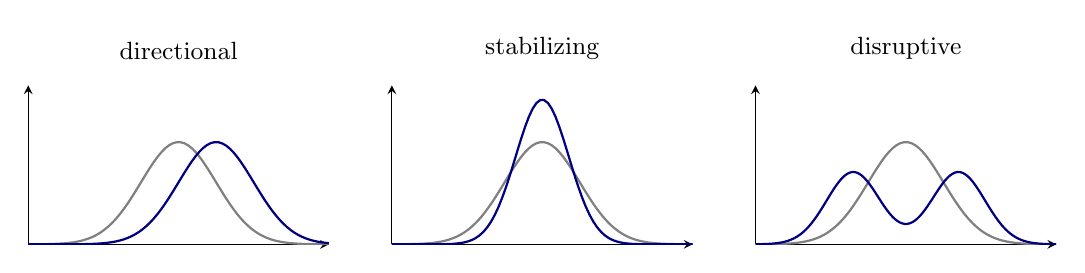
\begin{tikzpicture}
\begin{groupplot}[group style={group size=3 by 1,horizontal sep=8mm},width=5.4cm,height=3.6cm,
  ticks=none,xmin=-4,xmax=4,ymin=0,ymax=0.62,axis lines=left]
\nextgroupplot[title={\small directional}]
\addplot[gray,thick,domain=-4:4,samples=80]{exp(-x^2/2)/sqrt(2*pi)};
\addplot[NavyBlue,thick,domain=-4:4,samples=80]{exp(-(x-1)^2/2)/sqrt(2*pi)};
\nextgroupplot[title={\small stabilizing}]
\addplot[gray,thick,domain=-4:4,samples=80]{exp(-x^2/2)/sqrt(2*pi)};
\addplot[NavyBlue,thick,domain=-4:4,samples=80]{exp(-x^2/(2*0.5))/sqrt(2*pi*0.5)};
\nextgroupplot[title={\small disruptive}]
\addplot[gray,thick,domain=-4:4,samples=80]{exp(-x^2/2)/sqrt(2*pi)};
\addplot[NavyBlue,thick,domain=-4:4,samples=120]{0.5*exp(-(x-1.4)^2/(2*0.5))/sqrt(2*pi*0.5)+0.5*exp(-(x+1.4)^2/(2*0.5))/sqrt(2*pi*0.5)};
\end{groupplot}
\end{tikzpicture}

\small Grey: trait distribution before; blue: after. Directional: the mean moves. Stabilizing: intermediates favoured,
variance falls. Disruptive: both extremes favoured, variance rises, may split.
\end{center}

\subsection{The nature of selection}
\begin{chain}[: selection on individuals, evolution of populations]
\begin{enumerate}
\item An individual's genotype is fixed for life. It survives or dies, reproduces more or less, but does not change.
No finch's beak grew from cracking \emph{Tribulus}.
\item Selection therefore \emph{sorts} individuals; the \emph{population's} composition shifts as a result.
\item Selection acts on \textbf{phenotypes}, but evolution happens only if \textbf{allele frequencies} change, which
requires the phenotypic differences to be heritable. With $h^2=0$ the drought would still have killed the small-beaked
birds, but the next generation would have bounced back: no evolution.
\item So ``selection acts on phenotypes; genotypes get selected; genes get differentially transmitted'' (wrap-up slide 13),
and \textbf{natural selection is not evolution}: selection without heritability gives no evolution, and evolution also has
other causes (drift, mutation, migration, non-random mating: the broken HW assumptions).
\end{enumerate}
\end{chain}
``The mess that is natural selection'' (slide 10): genes $\to$ genotype $\to$ (with biotic and abiotic environment)
phenotype $\to$ selection $\to$ meiosis $\to$ fertilisation $\to$ genes, with \textbf{chance} at every step.

\begin{trap}[: heritability is not ``resemblance'']
``Obese children often have obese parents'' or ``long-winged birds have long-winged offspring'' does not show a genetic
basis: shared diet, island, rearing conditions or maternal effects produce resemblance too. A genetic basis needs a
common-garden or cross-fostering design, or crosses. And predicting a response needs differential fitness as well
(2022 end-sem Q4; 2024 end-sem Q2).
\end{trap}

\subsection{What selection is not}
\begin{itemize}
\item \textbf{Always behind}: it changes frequencies \emph{after} exposure; the 1978 finches were adapted to 1977, not to
what came next. It cannot anticipate; new mutations do not arise to meet needs; a population facing too-fast change may go
extinct.
\item \textbf{Not progressive}: organisms ``devolve'' as often as they evolve (parasites); adaptation proceeds by gain,
loss and modification of characters.
\item \textbf{Works with what is available}: pre-existing variation, co-opted structures (\textbf{preadaptations}); no grand
design, no perfection. \emph{Gambusia} mosquitofish: a large gonopodium attracts mates but hinders escape, so males in
high-predation populations have smaller ones: a \textbf{trade-off}, not an optimum.
\item \textbf{Yet new traits evolve}: mutation and recombination create new combinations, which selection sorts (Illinois
corn oil: from 4--6\,\% to $\sim$20\,\% in 100 generations, far beyond the starting range).
\end{itemize}

\subsection{One-locus selection (beyond the slides, but explains the past-paper items)}
Selection enters the HW cycle between zygote and adult: zygotes form at $p^2:2pq:q^2$, then survive with fitnesses
$w_{11},w_{12},w_{22}$:
\[
p'=\frac{p^2w_{11}+pq\,w_{12}}{\bar w},\qquad \bar w=p^2w_{11}+2pq\,w_{12}+q^2w_{22},\qquad
\Delta p=\frac{pq\,[\,p(w_{11}-w_{12})+q(w_{12}-w_{22})\,]}{\bar w}.
\]
\begin{chain}[: what the formula says]
\begin{itemize}
\item The factor $pq$: selection is slow when either allele is rare (little variation to act on).
\item A \textbf{recessive} favoured allele is invisible when rare (almost all copies sit in heterozygotes, HW property 5),
so it takes very long to start spreading. A \textbf{dominant} favoured allele spreads fast at first but stalls at the end,
because the last disfavoured recessive copies hide in heterozygotes. Additive alleles are fastest overall ($s=0.1$: 175
generations vs $\sim$1000).
\item \textbf{Overdominance} (heterozygote advantage, $w=1-s:1:1-t$): stable polymorphism at $p^*=t/(s+t)$; variation is
maintained (classic case: sickle-cell in malarial regions).
\item \textbf{Underdominance} (heterozygote disadvantage): an \emph{unstable} interior equilibrium; whichever allele starts
above it goes to fixation (a threshold, like the Allee effect).
\item \textbf{Breeder's equation} $R=h^2S$: only the heritable fraction of the selection differential is passed on.
\end{itemize}
\end{chain}

\begin{statements}
\begin{enumerate}[label=\arabic*.]
\item ``The finches' beaks deepened because birds needed to crack hard seeds.''
\F No individual changed; small-beaked birds died, and deep beaks were heritable.
\item ``Natural selection always requires mortality.''
\F Differences in reproduction alone suffice.
\item ``If a trait is under strong selection but has zero heritability, the population will still evolve, only more slowly.''
\F No evolution at all; the next generation returns to the old distribution.
\item ``Stabilizing selection shifts the mean toward the optimum and widens the distribution.''
\F It keeps the mean and narrows the distribution; disruptive selection widens it.
\item ``The reversal of selection in 1983 shows that the 1977 evolution was an error of measurement.''
\F Selection tracks a changing environment; reversals are expected (lesson 2).
\item ``Fossil sequences showing slow change mean evolution is slow.''
\F Fast zig-zags average out over the long spans a fossil bed mixes (lesson 3).
\item ``A new beneficial recessive allele spreads quickly because it is beneficial.''
\F It is almost never expressed while rare (it sits in heterozygotes), so selection barely sees it (2024 end-sem Q11).
\item ``Heterozygote advantage maintains both alleles in the population.''
\T Stable equilibrium at $p^*=t/(s+t)$.
\item ``Selection produces the variation it acts on.''
\F Mutation and recombination do; selection sorts.
\item ``Competition from \emph{G.\ magnirostris} changed the direction of selection on \emph{G.\ fortis} beaks.''
\T In 2004 it took the large seeds, so smaller beaks were favoured.
\end{enumerate}
\end{statements}

\begin{longans}[: ``Natural selection is not evolution. Discuss.'']
(1) Definitions: selection (differential survival/reproduction due to phenotype) vs evolution (change in allele/genotype
frequencies across generations). (2) Four postulates; Daphne Major tests each (numbers). (3) Selection acts on
individuals and phenotypes; evolution requires heritability ($h^2=0$ thought experiment; $R=h^2S$). (4) Other causes of
evolution (drift, mutation, migration, non-random mating). (5) Properties: always behind, not progressive, uses what is
available (\emph{Gambusia}), yet new traits arise. (6) Lessons: rapid, reversible, zig-zags look gradual.
\end{longans}

% ===================================================================
\section{Putting it all together}
% ===================================================================

\subsection{The wrap-up lecture's messages}
The final lecture (13 Nov) warns that its slides are ``not your summary sheet for the exams''; its chief messages, with
where each sits in these notes:
\begin{center}\small
\begin{tabularx}{\textwidth}{lX}
\toprule
theme & message\\\midrule
biology & many structural and temporal levels interact and change simultaneously: that causes the complexity (\S2)\\
modelling & useful, but never mistake the model for reality; mind its limitations (\S2, \S4)\\
population numbers & the strategy depends on problem, data and insight needed: no universal strategy (\S3, \S4)\\
complex systems & high-dimensional objects can have simple low-dimensional projections; a model with the expected behaviour
is not thereby appropriate (\S4)\\
applications & done properly, models inform policy and save lives; done badly, they harm (\S3, \S8)\\
competition & competitors often drive others extinct (water hyacinth in the Mula river at Dapodi); coexisting competitors
probably partition the niche, though it is often hard to show (\S5)\\
predation & in simple homogeneous systems prey are driven extinct; real systems are heterogeneous and both sides evolve: a
dynamic, ever-shifting equilibrium (\S6)\\
organism $\leftrightarrow$ environment & a two-way interaction, which is why ecosystems are hard to change (\S7)\\
conservation & very complex; needs inputs from many sources (\S8)\\
evolution & complex; much known, much to learn; work in progress, no major paradigm shift yet (\S9)\\
Hardy--Weinberg & ``the law is boring; the deviations are interesting''; even simple departures give counter-intuitive results (\S10)\\
selection & NS = differential survival and reproduction due to phenotype; NS is not evolution; evolution can be fast;
selection's effects are not always easy to predict (\S11)\\\bottomrule
\end{tabularx}
\end{center}

\subsection{Threads that cross chapters}
\begin{chain}[: one mathematics of thresholds]
\begin{itemize}
\item \textbf{Lakes}: vegetation--turbidity loop $\Rightarrow$ two states, folds, hysteresis.
\item \textbf{Allee effect}: positive density dependence $\Rightarrow$ extinction threshold $A$; harvest $\Rightarrow$ fold.
\item \textbf{Competition, unstable case}: neither species can invade $\Rightarrow$ saddle, priority effect.
\item \textbf{Underdominance}: heterozygote disadvantage $\Rightarrow$ unstable allele frequency.
\item \textbf{Passenger pigeon}: social facilitation $\Rightarrow$ MVP crossed while common.
\item \textbf{Wildebeest}: migration appears only above a tracking radius of $\sim$80\,km.
\end{itemize}
Common lesson: once past the threshold, reversing the original pressure does not restore the old state. Act before it, and
monitor the margin (resilience), not just the current state.
\end{chain}

\begin{chain}[: stability, three ways]
For a continuous model a fixed point is stable if the slope $f'(x^*)<0$ (logistic at $K$: $-r$). For a discrete map, if
$|g'(x^*)|<1$ (Ricker: $|1-r|<1$); losing stability at $g'=-1$ gives period doubling. For a linear matrix model, the zero
state is unstable when the dominant eigenvalue $\lambda>1$. In 2-D (competition, predator--prey) the Jacobian's trace and
determinant decide: trace $<0$ and determinant $>0$ means stable; purely imaginary eigenvalues (basic L--V) mean neutral.
\end{chain}

\begin{chain}[: chance at every level]
Demographic stochasticity (extinction of small populations), genetic drift ($H_t=H_0(1-1/2N_e)^t$), environmental
stochasticity, the integer lattice (chaos to cycles or extinction), founder bottlenecks in invaders, and chance in the
``mess'' of selection. Small numbers make all of them worse; large numbers average out only the demographic and genetic kinds.
\end{chain}

\begin{chain}[: top-down and bottom-up]
Hare--lynx: three trophic levels interact (Krebs). Lakes: nutrients (bottom-up) and fish $\to$ \emph{Daphnia} $\to$ algae
(top-down: biomanipulation, Lake Washington's second jump). Wildebeest: food-limited (bottom-up); zebra probably
predation-limited (top-down). Volterra's principle: indiscriminate killing helps prey.
\end{chain}

\subsection{Past-paper topics outside this year's slides}
Several past papers (2021--2025) asked about topics that are not on this year's slides; they come from the self-study items
of lecture 2 (temperature, biogeochemical cycles) and from earlier runs of the course (ageing). They are summarised here as
general knowledge, in case they reappear.

\textbf{Ageing (evolutionary theories).} Both rest on the \textbf{declining force of selection with age}: few individuals
survive to old age, so effects acting late matter little to fitness.
\begin{itemize}
\item \textbf{Mutation accumulation} (Medawar): late-acting deleterious mutations are weakly selected against and
accumulate by mutation and drift; ageing is their summed effect. Predicts increased genetic variance in late-life traits.
\item \textbf{Antagonistic pleiotropy} (Williams): alleles with early benefits and late costs are actively \emph{favoured};
ageing is the price of early vigour. Predicts negative genetic correlation between early and late fitness.
\item \textbf{Extrinsic mortality} sets the strength of selection on late life: low extrinsic mortality (captivity, flight,
shells) $\Rightarrow$ selection maintains late fitness $\Rightarrow$ slower ageing. So zoo-bred rabbits evolve to age
\emph{slower}; zoo rabbits released to the wild evolve to age \emph{faster}. A deleterious allele acting at 35--55 is purged
less than one acting at 15--35.
\item Birds outlive same-sized mammals despite higher metabolic rates: evidence against the \textbf{rate-of-living} theory.
\item ``Programmed death for the good of the species'' relies on group selection (a cheater allele that keeps its carrier
alive would spread) and is contradicted by the observation that wild animals rarely live long enough to age.
\end{itemize}

\textbf{Nutrient cycles and agriculture.} Energy flows, matter cycles: reservoirs and fluxes; gaseous cycles (C, N) vs
sedimentary (P, S). \textbf{Nitrogen fixation}: N$_2\to$ NH$_3$/NH$_4^+$ by nitrogenase (\emph{Rhizobium} in legume
nodules, cyanobacteria), lightning, industry. \textbf{Nitrification}: NH$_4^+\to$ NO$_2^-\to$ NO$_3^-$ by aerobic
bacteria. \textbf{Denitrification}: NO$_3^-\to$ N$_2$O $\to$ N$_2$ by anaerobic bacteria; returns N to the air.
\textbf{Crop rotation} alternates crops (e.g.\ with N-fixing legumes) on one field; \textbf{slash-and-burn} (\emph{jhum})
releases nutrients as ash, farms a few years, then leaves a long fallow; sustainable only with long fallows and low density.
\textbf{Mean residence time} = stock/throughput flux. Phosphorus, unlike N, has no gaseous phase and is relatively
immobile in soil (hence the past question about advising a king with P-deficient crops: return P via manure, bones, ash,
river silt).

\textbf{Temperature} (Begon \& Townsend, self-study). Rates rise roughly exponentially with temperature: $Q_{10}$, the factor
per 10\,°C, often $\approx2$. Development is summarised by \textbf{day-degrees} above a threshold. The
\textbf{temperature--size rule}: final size falls as rearing temperature rises. \textbf{Endotherms} hold body temperature
nearly constant (flat line against environment) at high energy cost; \textbf{ectotherms} track environmental temperature
(near the line $T_b=T_{env}$), adjusted by basking and shade-seeking; insects can warm up by basking or shivering their
flight muscles. Freezing removes liquid water from cells, so cold injury resembles drought and salinity stress.

\begin{trap}
These items are not in this year's slides; if a question uses them, reason from the principle (declining force of selection;
mass balance of nutrients; rate--temperature relations) rather than recalled detail.
\end{trap}

% ===================================================================
\section{Catalogue of examples: where, and what each shows}\label{sec:examples}
% ===================================================================
Every case study, experiment and data set used in the course, with the place or organism, what was observed, and the
idea it is used to support. Statement MCQs often name an example and ask what it demonstrates, so learn the right-hand
column as one sentence per row.

{\small
\renewcommand{\arraystretch}{1.3}
\begin{longtable}{>{\raggedright\arraybackslash}p{0.19\textwidth}>{\raggedright\arraybackslash}p{0.22\textwidth}>{\raggedright\arraybackslash}p{0.27\textwidth}>{\raggedright\arraybackslash}p{0.24\textwidth}}
\toprule
example & where / who & what is seen & what it shows\\\midrule
\endhead
\multicolumn{4}{l}{\textbf{EE01 Biology and ecological thinking}}\\
Wildebeest migration & Serengeti--Mara, Tanzania/Kenya; $\sim$1.2--1.3 million & $\sim$1500\,km/yr loop following green grass & proximate vs ultimate questions; emergence\\
Wildebeest muscle & Curtin et al.\ 2018 (Botswana animals) & 62.6\,\% efficient vs cow 41.8, mouse 34 & a ``how'' adaptation: less fuel, far less waste heat\\
Synchronous calving & Serengeti plains, mid-Feb & 250{,}000 calves in $\sim$3 weeks ($\sim$80\,\%) & predator satiation lowers the fraction lost\\
Precocial calves & Serengeti & stand in $\sim$6 min; topi/hartebeest much slower & a moving herd cannot carry helpless young\\
Opposing gradients & Holdo et al.\ 2009 model & rain rises SE$\to$NW, fertility falls; migration only with tracking $\gtrsim$80\,km & migration follows quality; a threshold\\
Mara drownings & Subalusky et al.\ 2017 & $\sim$6000 drown/yr; carcasses and bones feed the river & animals move nutrients; two-way organism--environment link\\
Rinderpest and fire & Serengeti, 1960s on & herd surged, grazing removed fuel, fire fell, trees recovered & trophic cascade from a virus to a landscape\\
Why so many & Hopcraft et al.\ 2015 & migrants $\gg$ residents; zebra $6\times$ fewer & strong inference by comparison; refuge + ephemeral resource + connectivity\\
\midrule
\multicolumn{4}{l}{\textbf{EE02 Structured populations}}\\
\emph{Phlox drummondii} & annual plant; Leverich \& Levin 1979 & cohort of 996; 84\,\% die before day 299; $R_0=2.4177$ & cohort life table; unlimited growth absurd\\
Dall sheep & Murie; 608 skulls & static life table; type I curve & static life tables; survivorship types\\
Mackerel, \emph{Leander}, \emph{Cleome} & Molles & $>$999{,}990 of $10^6$ mackerel eggs die in 70 days & type III survivorship\\
Robin, white-crowned sparrow & Molles & constant proportional mortality & type II survivorship\\
Slide-16 Leslie model & hypothetical, 4 classes & zig-zag, then $\lambda=1.05082$, SAD (0.635, 0.302, 0.057, 0.005) & convergence to a stable age distribution\\
Loggerhead turtle & SE USA; Crouse 1987, Crowder 1994 & $\lambda=0.9516$; large juveniles highest elasticity; perfect egg survival still $\lambda<1$ & stage models, elasticity, where to act\\
TEDs & shrimp trawls; India 1996 law & 5.7\,kg by-catch/kg shrimp; $\sim$70\,yr (seasonal) vs $\sim$33\,yr (full) for 10$\times$ & intervention at the sensitive stage; slow recovery\\
White oak & Illinois forest & many young trees & a replacing population\\
Rio Grande cottonwood & dammed rivers, SW USA & 40--50-yr-olds, no recruitment & dams removed floods seedlings need\\
Large cactus finch & Genovesa, Galápagos & gaps in age structure after droughts & pyramids record history\\
Sweden, Hungary, Rwanda & UN 2020 data & $r=0$, $-0.003$, $+0.027$ & pyramid shape vs growth; doubling 25.7\,yr\\
\midrule
\multicolumn{4}{l}{\textbf{EE03 Dynamics and chaos}}\\
Locust record & China, oracle bone; 1910-yr index & irregular outbreaks & prediction of numbers is old and hard\\
US census; rotifer \emph{Brachionus} & Pearl \& Reed 1920; Yoshinaga 2001 & S-shaped rise, plateau with fluctuation & logistic as a rough fit\\
Fibonacci's rabbits & Pisano, 1202 & ratio $\to1.618$ & first population model (a Leslie matrix)\\
Ricker map & model & stable $\to$ 2, 4, 8 cycles $\to$ chaos (2.69) & overcompensation; period doubling\\
Hassell et al.\ 1976 & 24 insect populations & 22 monotone damping & ``natural populations are simple''---the puzzle\\
Henson et al.\ 2001 & integerised models (\emph{Science}) & chaos becomes cycles or extinction & lattice effect\\
Turchin \& Taylor 1992 & 14 insect + 22 vertebrate series & full spectrum incl.\ chaos & simple models biased to stability\\
\midrule
\multicolumn{4}{l}{\textbf{EE04 Competition and invasions}}\\
Gause, \emph{Paramecium} & lab cultures & \emph{P.\ aurelia} excludes \emph{P.\ caudatum} & competitive exclusion\\
Tilman's diatoms & \emph{Asterionella}, \emph{Synedra}; silicate & one displaces the other & one limiting resource, one winner ($R^*$)\\
Kerala invaders & 2018--19 floods; 44 rivers, 53 reservoirs & 28 alien fish + 4 weeds, 7 established (arapaima, alligator gar) & invaders as super-competitors\\
Water hyacinth & Kerala, Assam, West Bengal; Mula river (Pune) & crafts, sarees from a pest & control and use of invaders\\
Asian carps; \emph{Caulerpa} & Great Lakes; Mediterranean & self-study & invasions\\
\emph{P.\ caudatum} / \emph{P.\ bursaria} & Gause & feed at top vs bottom; coexist & spatial partitioning\\
Connell's barnacles & rocky intertidal shore & \emph{Chthamalus} high (Balanus desiccates), \emph{Balanus} middle, predation low & physical limits + competition; realised $<$ fundamental niche\\
Spiny mice & Israel deserts & golden mouse turns nocturnal when common mouse removed & temporal partitioning induced by competition\\
Galápagos ground finches & several islands & beak depth differs more in sympatry & character displacement\\
Park's \emph{Tribolium} & flour beetles, 6 climates & winner flips with temperature/humidity; bigger $K$ can lose & conditional outcome; $\alpha$ matters, not just $K$\\
\midrule
\multicolumn{4}{l}{\textbf{EE05 Predation}}\\
Hare--lynx & Hudson's Bay Co.\ furs, Canada (Elton 1924) & $\sim$10-yr cycles, lynx lagging & cycles; intrinsic vs extrinsic\\
Krebs et al.\ 1995 & boreal forest, 1-km$^2$ blocks, 8 years & predators out $\times2$, food $\times3$, both $\times11$ & three trophic levels interact\\
Gause, \emph{Didinium} & lab & extinction; refuge: predator dies; immigration: cycles & simple systems collapse\\
Huffaker's mites & 120 oranges, barriers & 3 oscillations in $\sim$6 months & heterogeneity + dispersal: metapopulation\\
Yellow-winged darter & dragonfly & conspicuous colour & aposematism\\
Dead-leaf mantis, frogmouth, lantern fly & various & background matching & crypsis\\
Drone fly / honey bee & & harmless mimic & Batesian mimicry\\
\emph{Heliconius} & Neotropical butterflies & shared pattern, all distasteful & Müllerian mimicry\\
Opossum; moths; mobbing birds; aphids & & play dead; startle; group defence; alarm pheromone & behavioural defences\\
Skunk, bombardier beetle & & toxic sprays & chemical defence (needs warning colour)\\
\midrule
\multicolumn{4}{l}{\textbf{EE06 Lakes}}\\
Schöhsee vs Lake Constance & Germany & P says meso/eu; oxygen says the opposite & morphometry; one criterion misleads\\
Caspian Sea 2003; Lake Erie & & eutrophication of huge waters & not only small lakes\\
Lake Washington & Seattle; Edmondson & sewage $\to$ ``Lake Stinko''; diversion 1968; \emph{Daphnia} 1976: 1$\to$3--4$\to$10\,m & reversal; food web decides final clarity\\
Lake Constance recovery & Central Europe & $P_{tot}$ 6 $\to$ 87 $\to$ 8\,µg/L & tertiary treatment, P-free detergents work\\
Schlachtensee & Berlin & lagging recovery & sediment P, slow water exchange\\
Lake Veluwe & Netherlands; Scheffer 2001 & charophytes collapse late 1960s, return 1990s at much lower P & alternative states, hysteresis\\
18 Dutch lakes & Meijer et al.\ 1999 & transparency up after fish removal & biomanipulation\\
Global P load & 2018 review & 1.5\,Tg/yr; China 30\,\%, India 8\,\% & scale of the problem\\
Aral Sea & Central Asia & shrunk by water policy & bad policy threatens fresh water\\
\midrule
\multicolumn{4}{l}{\textbf{EE07 Conservation}}\\
Muir / Pinchot (Brandis) / Leopold & USA; Indian forestry & preserve / use wisely / land ethic & three conservation ethics\\
Passenger pigeon & eastern N.\ America; 1878 / 1914 & no rebound after hunting ended & social facilitation + habitat loss; MVP crossed while common\\
Murray et al.\ 2017 & pigeon genomes & low diversity shaped by selection & genetic role ``unknown''\\
Project Tiger & India, 1973; 9 reserves & 1827 $\to$ $>$4000 $\to$ reversals $\to$ 2967 (2018) & politics, design, counting\\
Sariska & Alwar, Rajasthan & all tigers lost to poaching & reversals; reserves $\neq$ tigers\\
Camera traps & Karanth \& Nichols; Nagarahole & stripes ID; $\hat N=C/\hat p$; pugmarks failed & detection-corrected estimates\\
Elephants; lemon trees & railways; Assam & collisions; citrus barrier & human--animal conflict, local solutions\\
SLOSS (Box 11.1) & Hunter \& Gibbs & nested: 1 large wins; un-nested: several small win & no universal reserve rule\\
Manyara--Tarangire; Chitwan & Tanzania; Nepal & migration corridor; grass-cutting access & connectivity; people management\\
\midrule
\multicolumn{4}{l}{\textbf{EE08 Evolution}}\\
Western Ghats, Andamans, Eaglenest & India & thousands of species & diversity to be explained\\
Tonguestones; mammoths & Steno; Cuvier & fossils are organisms; species go extinct & the Earth changes; extinction\\
Watchmaker & Paley & complexity implies design & the argument Darwin had to answer\\
Homology; Wallace line & arm/wing/flipper; Indonesia & shared bones; faunal break & descent with modification\\
Jenkin's blending & Fleeming Jenkin & variance halves per generation & inheritance objection\\
Rat maternal care & Weaver et al.\ 2004 & licking demethylates GR promoter; calmer adults; cross-fostering reverses & environment alters epigenome\\
Romanian orphans; abuse & Sheridan 2012; McGowan & lasting brain/stress effects; GR methylation & same in humans\\
Vinclozolin & rats & disease in $\ge$4 male generations & transgenerational epigenetic inheritance\\
Toadflax \emph{Linaria} & Cubas et al.\ 1999 & peloric form = methylated \emph{Lcyc}, heritable & epimutation\\
\emph{Elysia chlorotica} & sea slug + alga \emph{Vaucheria} & keeps plastids; HGT claim not supported & HGT (retracted case)\\
\midrule
\multicolumn{4}{l}{\textbf{EE09 Hardy--Weinberg}}\\
Pueblo MN & Templeton & 83/46/11, $p=0.757$, $\chi^2=1.59$ & HW test, fits\\
Brachydactyly (Yule) & Hardy 1908 & ``should be 3:1'' & family ratio $\neq$ population frequency\\
Acid phosphatase & 178 English people & no CC seen; 0.27 expected & rare genotypes absent under HW\\
PKU, albinism, PTC & & 1/11000, 1/10000, 30\,\% & carrier estimates; rare alleles hide in heterozygotes\\
Icelandic sheep, Shorthorn cattle, Gm, MN & practice set & yellow fat; roan; Swedish counties & conditioning; codominance; $2pq$\\
\midrule
\multicolumn{4}{l}{\textbf{EE10 Selection}}\\
\emph{Geospiza fortis} & Daphne Major, Galápagos; Grants since 1973 & 1977 drought: 84\,\% died, deeper beaks; $h^2=0.65$; 1983 El Niño reversed; 2004 + \emph{G.\ magnirostris}: smaller & all four postulates; fast, reversible evolution\\
\emph{Tribulus cistoides} & Daphne Major & hard fruits only deep beaks crack & agent of selection\\
\emph{Gambusia} & mosquitofish & big gonopodium attracts mates, slows escape & trade-offs; no perfection\\
Illinois corn oil & since 1896 & 4--6\,\% $\to$ $\sim$20\,\% oil & selection beyond the original range\\
Sickle-cell & malarial regions & heterozygote advantage & balanced polymorphism\\
\bottomrule
\end{longtable}
}

% ===================================================================
\section{Glossary of terms}\label{sec:glossary}
% ===================================================================
{\small
\setlength{\columnsep}{1.4em}
\begin{multicols}{2}
\begin{description}[leftmargin=0pt,itemsep=2pt,font=\bfseries]
\item[Adaptation] A trait shaped by natural selection that suits the environment; Darwin's Inf 3.
\item[Adaptive force (Lamarck)] Force fitting organisms to local conditions by use/disuse and inheritance of acquired characters.
\item[Age pyramid] Bar chart of age-class shares, males and females back to back; base broadens with $\lambda$.
\item[Allee effect] Per-capita growth falling as density falls; strong form has an extinction threshold $A$.
\item[Allele frequency] Share of gene copies of an allele: $p=P+Q/2$ (always true).
\item[Alternative stable states] Two or more stable states under the same conditions (clear vs turbid shallow lake).
\item[Antagonistic pleiotropy] Ageing theory: alleles with early benefits and late costs are favoured.
\item[Aposematism] Conspicuous warning signal of a defended prey, letting predators learn.
\item[Batesian mimicry] Harmless mimic copies a defended model's signal; protected only while rarer than the model.
\item[Bifurcation diagram] Long-run values visited against a parameter; number of points = period.
\item[Biomanipulation] Reducing planktivorous fish so grazers clear the water; a push across a threshold.
\item[Blending inheritance] Offspring = mid-parent value; halves heritable variance each generation (Jenkin).
\item[Buffer zone] Partly used land around a reserve core; holds prey, dispersal routes, distance from people.
\item[Carrying capacity ($K$)] Density at which the realised per-capita growth rate is zero.
\item[Catalepsis] Playing dead (thanatosis), e.g.\ the opossum.
\item[Causal loop diagram] Network of signed effects; the loop sign is the product of link signs.
\item[Character displacement] Related species differ \emph{more} where they co-occur than where apart.
\item[Chaos (deterministic)] Bounded, aperiodic dynamics with sensitive dependence on initial conditions; no noise involved.
\item[Clinograde / orthograde] Summer O$_2$ profile falling to zero with depth (eutrophic) / staying high (oligotrophic).
\item[Cohort] Individuals born in the same period, followed together.
\item[Cohort life table] Record of a cohort's survivorship $l_x$ and fecundity $m_x$ by age.
\item[Competition] Use or defence of a resource that reduces its availability to others; non-trophic.
\item[Competitive exclusion principle] No two species with the same niche (one limiting resource) can coexist (Gause).
\item[Complexifying force (Lamarck)] Force moving lineages up a master plan toward greater complexity.
\item[Contest / scramble competition] Resource shared out so more parents never mean fewer offspring / split so finely that crowding lowers output (overcompensation).
\item[Crypsis] Avoiding detection by matching the background.
\item[Cultural eutrophication] Nutrient enrichment of waters by human activity.
\item[Demographic stochasticity] Chance variation in births, deaths, sex ratio; relative size $\sim1/\sqrt N$.
\item[Density dependence] Per-capita rates changing with density (negative: crowding; positive: Allee).
\item[Descent with modification] All species are branches of one tree, changed from common ancestors.
\item[Detection probability ($p$)] Chance an animal present is counted; $\hat N=C/\hat p$.
\item[Directional / stabilizing / disruptive selection] Favours one extreme (mean shifts) / intermediates (variance falls) / both extremes (variance rises).
\item[Dominant eigenvalue ($\lambda$)] Largest-modulus eigenvalue of a projection matrix; long-run growth factor.
\item[Dystrophic lake] Low conductivity, brown humic water.
\item[Ecology] Study of interactions of organisms with their biotic and abiotic environment, explaining distribution and abundance.
\item[Effective population size ($N_e$)] Size of an ideal population with the same drift rate; usually $<$ census $N$.
\item[Elasticity] Proportional change in $\lambda$ per proportional change in a matrix entry; elasticities sum to 1.
\item[Emergence] Properties of a whole not found in its parts (a migration, a traffic jam).
\item[Environmental stochasticity] Shocks affecting all individuals together; does not average out with $N$.
\item[Epigenetic inheritance] Transmission of gene-expression states (e.g.\ methylation) without DNA sequence change.
\item[Ergodicity (demographic)] A primitive matrix population forgets its initial structure.
\item[Eutrophic] Highly productive, green, often with anoxic hypolimnion; $P_{tot}$ 30--100\,µg\,L$^{-1}$.
\item[Extended Evolutionary Synthesis] Proposed extension of the MS: epigenetics, inheritance of some acquired states, HGT, evo-devo.
\item[Fitness] Relative contribution to the next generation (survival $\times$ reproduction) of a genotype or phenotype.
\item[Fractal] Self-similar at many scales (the bifurcation diagram).
\item[Functional response] Prey eaten per predator as a function of prey density (Holling II saturates at $1/h$).
\item[Fundamental / realised niche] Where a species could persist alone / where it actually does with enemies and competitors.
\item[Genetic drift] Random change in allele frequency from sampling; strongest in small populations.
\item[Genetic stochasticity] Drift, loss of heterozygosity and inbreeding depression in small populations.
\item[Hardy--Weinberg equilibrium] $p^2:2pq:q^2$ with constant frequencies under no evolutionary forces.
\item[Heritability ($h^2$)] Fraction of trait variation that is (additively) genetic; sets response $R=h^2S$.
\item[Horizontal gene transfer] Genes moving between contemporaneous organisms, even across species.
\item[Hypolimnion / epilimnion] Cold dark bottom layer / warm mixed top layer of a stratified lake.
\item[Hysteresis] The return path differs from the outward path; recovery needs a larger reversal.
\item[Inbreeding depression] Fitness loss from mating among relatives exposing deleterious recessives.
\item[Internal loading] Phosphorus release from (anoxic) sediments; makes eutrophication self-accelerating.
\item[Intrinsic / extrinsic cause of cycles] Generated by interacting populations / imposed from outside (weather, sunspots).
\item[Irreducible / primitive matrix] Life-cycle graph connected / loop lengths with gcd 1; together they guarantee a SAD.
\item[Isocline (zero-growth)] Curve where one species' growth rate is zero.
\item[Lattice effect] Integer counts with a bound give finitely many states, so chaos becomes cycles or extinction.
\item[Lefkovitch matrix] Stage-structured projection matrix with stay ($P$), grow ($G$) and fecundity ($F$) entries.
\item[Leslie matrix] Age-structured projection matrix: fecundities in row 1, survivals on the sub-diagonal.
\item[Limit cycle] Isolated periodic orbit with fixed amplitude; attracts nearby orbits (unlike neutral L--V cycles).
\item[Lyapunov exponent] Average exponential rate of divergence of nearby orbits; $>0$ means chaos.
\item[Macroevolution / microevolution] Change above the species level over long times / change in trait values or allele frequencies within populations.
\item[Mark--recapture] Estimating $N$ from recapture rates of marked animals ($\hat N=Mn/m$).
\item[Metapopulation] Set of local populations linked by dispersal, persisting through extinction and recolonisation.
\item[Minimum dynamic area] Smallest reserve area holding a mosaic of disturbance and succession patches.
\item[Minimum viable population (MVP)] Smallest size giving an acceptable persistence probability over a stated time.
\item[Modelling relation (Rosen)] Encode nature into a formal system, infer, decode; good if it matches causal entailment.
\item[Modern Synthesis] 1930s--50s union of Darwin and Mendelian genetics: selection on particulate variation; micro $\to$ macro.
\item[Müllerian mimicry] Several defended species share one warning signal.
\item[Mutation accumulation] Ageing theory: late-acting deleterious mutations escape selection and accumulate.
\item[Natural selection] Differential survival and reproduction of individuals due to phenotypic differences.
\item[Net reproductive rate ($R_0$)] Mean lifetime offspring per newborn, $\sum l_xm_x$.
\item[Neutral stability] Displaced system stays at its new state (HW allele frequency; L--V orbits).
\item[Niche (persistence / utilisation)] Conditions allowing positive growth (Hutchinson) / what the species actually uses (MacArthur, Levins).
\item[Niche partitioning] Separation of resource use in space, time, morphology or conditions, allowing coexistence.
\item[Oligotrophic] Low productivity, clear water, oxygenated depths; $P_{tot}$ 5--10\,µg\,L$^{-1}$.
\item[Overcompensation] Crowding cuts output so much that the population overshoots its equilibrium.
\item[Overdominance / underdominance] Heterozygote fitter (stable polymorphism) / less fit (unstable equilibrium).
\item[Period doubling] Successive births of 2-, 4-, 8-cycles as a parameter rises; route to chaos.
\item[Phase plane] Plot of one population against another, with isoclines and trajectories.
\item[Population] Similar individuals inhabiting a defined space at a given time.
\item[Population thinking] Every individual is unique; the mean is an abstraction (vs essentialism).
\item[Preadaptation] Existing trait co-opted for a new use.
\item[Predation] Eating all or part of another organism (herbivory, carnivory, parasitoidism, parasitism, cannibalism).
\item[Predator satiation] Prey appearing in numbers far beyond predators' capacity, lowering the fraction taken.
\item[Priority effect] The first established competitor excludes the other (unstable L--V case).
\item[Proximate / ultimate cause] How a trait works (mechanism) / why it exists (evolutionary benefit).
\item[$R^*$] Resource level at which a species' growth balances losses; lowest $R^*$ wins.
\item[Rabinowitz rarity] Range $\times$ habitat tolerance $\times$ local population: one common, seven rare types.
\item[Regime shift] Abrupt change to a contrasting state when a threshold is crossed.
\item[Relaxation time] Time scale of return to equilibrium after a disturbance ($1/r$ for the logistic).
\item[Reproductive value ($v$)] Expected future contribution of an individual of a given stage (left eigenvector).
\item[Resilience] Size of the disturbance a state can absorb without shifting (depth of its basin).
\item[Saltationism] Evolution by large sudden jumps rather than gradual change.
\item[Sensitivity] Absolute change in $\lambda$ per absolute change in a matrix entry, $v_iw_j/\mathbf v\cdot\mathbf w$.
\item[SLOSS] Single large or several small reserves; depends on nestedness of species lists.
\item[Stable age (stage) distribution] Constant class proportions reached under fixed vital rates; dominant right eigenvector.
\item[Structural instability] Qualitative behaviour changes under any small change in the equations (basic L--V).
\item[Survivorship curve] $\log l_x$ against age; types I (late loss), II (constant proportion), III (early loss).
\item[Trophic continuum] Modern view of lake trophic states as ranges of $P_{tot}$ at spring circulation.
\item[Turtle excluder device (TED)] Escape hatch in trawl nets protecting large juvenile and older turtles.
\item[Volterra's principle] Killing predator and prey at the same rate raises mean prey and lowers mean predators.
\end{description}
\end{multicols}
}

% ===================================================================
\section{Equation sheet}\label{sec:equations}
% ===================================================================
Each row gives the relation, what it means, and the condition or catch an MCQ would test.

{\small
\renewcommand{\arraystretch}{1.45}
\begin{longtable}{p{0.40\textwidth}p{0.53\textwidth}}
\toprule
relation & meaning, condition, catch\\\midrule
\endhead
\multicolumn{2}{l}{\textbf{Structured populations (EE02)}}\\
$N_{t+1}=N_t+B-D+I-E$ & population bookkeeping\\
$l_x=n_x/n_0$,\quad $R_0=\sum_x l_xm_x$ & lifetime offspring per newborn; per \emph{generation}\\
$\ln n_x=\ln n_0+x\ln(1-q)$ & constant risk $q$ is a straight line on a log axis (type II)\\
$T=\sum x\,l_xm_x/R_0$,\quad $r\approx\ln R_0/T$ & generation time; approximate growth rate (beyond slides)\\
$\mathbf n_{t+1}=\mathbf L\mathbf n_t$ & Leslie: row 1 fecundities, sub-diagonal survivals\\
$\mathbf n_t\to c\lambda^t\mathbf w$ & long run: growth by $\lambda$, shape $\mathbf w$ (SAD); needs primitive matrix\\
$1=\sum_x F_xl_x\lambda^{-x}$ & Euler--Lotka; one positive root; $\lambda>1\iff R_0>1$\\
$w_{x+1}/w_x=P_x/\lambda$ & SAD class ratios; larger $\lambda$ $\Rightarrow$ broader pyramid base\\
$P_i+G_i=\sigma_i$ & stage matrix: stay + grow = annual survival\\
$G=\sigma\gamma$,\ $\gamma=\dfrac{x^{T-1}(1-x)}{1-x^T}$,\ $x=\sigma/\lambda$ & graduation from a stage lasting $T$ years\\
$s_{ij}=\dfrac{v_iw_j}{\mathbf v\cdot\mathbf w}$,\quad $e_{ij}=\dfrac{a_{ij}}{\lambda}s_{ij}$,\ $\sum e_{ij}=1$ & sensitivity (absolute) and elasticity (proportional); rank with elasticity\\
\midrule
\multicolumn{2}{l}{\textbf{Growth and chaos (EE03)}}\\
$N_t=\lambda^tN_0$,\quad $\lambda=1+b-d+i-e$ & discrete exponential (``first law'')\\
$N=N_0e^{rt}$,\quad $\lambda=e^r$ & continuous exponential; $r\approx b-d$ only for small rates\\
$t_d=\ln2/r$;\quad halving $\ln2/|r|$ & independent of $N$\\
$\dot N=rN(1-N/K)$ & logistic; per-capita rate falls linearly to 0 at $K$\\
$N(t)=\dfrac{K}{1+\frac{K-N_0}{N_0}e^{-rt}}$ & solution; inflection at $K/2$; max $\dot N=rK/4$; relaxation time $1/r$\\
$t_{K/2}=\ln[(K-N_0)/N_0]/r$ & time to reach half of $K$\\
$N_{t+1}=N_t[1+r(1-N_t/K)]$ & discrete logistic (logistic map with $a=1+r$)\\
$n_{t+1}=n_te^{r(1-n_t/K)}$,\quad $g'(K)=1-r$ & Ricker: stable $0<r<2$ (monotone $r<1$); 2-cycle at 2; 4 at 2.5265; 8 at 2.6564; chaos from 2.6924; $K$ only rescales\\
$|g'(x^*)|<1$ & stability of a fixed point of a map\\
$\delta_t\approx\delta_0e^{\Lambda t}$;\quad $t_{\text{horizon}}\approx\ln(\text{range}/\delta_0)/\Lambda$ & chaos: horizon grows only logarithmically with precision\\
$N_{t+1}=\lambda N_t(1+aN_t)^{-\beta}$ & Hassell; $N^*=(\lambda^{1/\beta}-1)/a$\\
$f'(N^*)=1-\beta(1-\lambda^{-1/\beta})$ & $\beta\le1$: always monotone (contest); instability needs large $\beta$ and $\lambda$\\
$\dot N=rN(t)[1-N(t-\tau)/K]$ & delayed logistic; cycles when $r\tau>\pi/2$ (beyond slides)\\
\midrule
\multicolumn{2}{l}{\textbf{Competition (EE04)}}\\
$\dot N_1=\dfrac{r_1N_1(K_1-N_1-\alpha_{12}N_2)}{K_1}$ & L--V; $\alpha_{12}$ = effect of 2 \emph{on} 1 in species-1 equivalents\\
$N_1=K_1-\alpha_{12}N_2$;\ $N_2=K_2-\alpha_{21}N_1$ & isoclines; intercepts $K_1, K_1/\alpha_{12}$ and $K_2, K_2/\alpha_{21}$\\
$\alpha_{12}<K_1/K_2$ and $\alpha_{21}<K_2/K_1$ & stable coexistence (each invades the other); implies $\alpha_{12}\alpha_{21}<1$\\
$N_1^*=\dfrac{K_1-\alpha_{12}K_2}{1-\alpha_{12}\alpha_{21}}$,\ $N_2^*=\dfrac{K_2-\alpha_{21}K_1}{1-\alpha_{12}\alpha_{21}}$ & coexistence equilibrium (only if both positive)\\
$R^*=\dfrac{mk}{\mu-m}$ & Monod break-even resource; lowest $R^*$ wins\\
$\alpha=\exp(-d^2/4\sigma^2)$ & niche overlap of Gaussian utilisation curves (illustration)\\
\midrule
\multicolumn{2}{l}{\textbf{Predation (EE05)}}\\
$\dot H=rH-pHP$,\ $\dot P=apHP-mP$ & L--V predator--prey\\
$H^*=m/(ap)$,\quad $P^*=r/p$ & prey level set by predator traits; predator level by prey growth\\
$V=apH-m\ln H+pP-r\ln P$ & conserved: neutral closed orbits\\
$T\approx2\pi/\sqrt{rm}$ & small-cycle period; predator lags by $\sim$\,quarter cycle\\
$\dot H=rH(1-H/K)-pHP$;\ $P^*=\frac rp(1-\frac{H^*}{K})$ & logistic prey: stable spiral; needs $K>m/(ap)$\\
$r\to r-\delta,\ m\to m+\delta$ & Volterra's principle: prey up, predators down\\
$g(N)=\dfrac{aN}{1+ahN}$ & Holling type II; max $1/h$; half-max at $N=1/(ah)$\\
$\dot p=cp(1-p)-ep$,\quad $p^*=1-e/c$ & Levins metapopulation; persists only if $c>e$\\
\midrule
\multicolumn{2}{l}{\textbf{Lakes (EE06)}}\\
$P_{tot}$ classes $<5,\ 5\text{--}10,\ 10\text{--}30,\ 30\text{--}100,\ >100$ & µg\,L$^{-1}$ at spring circulation\\
$P_L=1.55\,[P_{in}/(1+\sqrt{\tau_w})]^{0.82}$ & longer retention $\Rightarrow$ more sedimentation, lower $P_L$\\
$\dot x=a-bx+r\dfrac{x^p}{x^p+h^p}$ & Box 1; bistable iff $\max rf'>b$; folds where $rf'(x)=b$\\
loop sign $=\prod$ link signs & positive: reinforcing; negative: balancing\\
\midrule
\multicolumn{2}{l}{\textbf{Conservation (EE07)}}\\
$P_{\text{ext}}=(d/b)^{N_0}$ & extinction risk even when $b>d$\\
$T_{\text{ext}}\sim e^{K\ln(b/d)}$ & persistence time grows exponentially with $K$\\
$H_t=H_0(1-1/2N_e)^t$ & heterozygosity loss by drift; half-life $\approx1.39N_e$\\
$N_e=4N_mN_f/(N_m+N_f)$ & effective size with unequal sex ratio\\
$\dot N=rN(N/A-1)(1-N/K)$ & strong Allee effect; 0 and $K$ stable, $A$ unstable\\
$\hat N=C/\hat p$ & count corrected for detection\\
$\hat N=Mn/m$;\ Chapman $\frac{(M+1)(n+1)}{m+1}-1$ & mark--recapture (closed population, equal catchability)\\
$p^*=1-(1-p)^K$ & caught at least once in $K$ occasions\\
\midrule
\multicolumn{2}{l}{\textbf{Evolution, HW and selection (EE08--EE10)}}\\
$V_t=V_0/2^t$ & blending inheritance destroys variance (Jenkin)\\
$p=P+Q/2$,\quad $q=R+Q/2$ & allele frequencies from genotypes, always valid\\
$p^2:2pq:q^2$,\quad $p'=p$ & HWE; one generation (two if sexes differ); neutral\\
$2pq\le\tfrac12$;\quad $H=1-\sum p_i^2\le 1-1/k$ & maximum heterozygosity\\
$(p_1+\dots+p_k)^2$ & $k$ alleles: $p_i^2$ and $2p_ip_j$\\
$\hat q=\sqrt{\text{freq(aa)}}$, carriers $2pq$ & recessive trait; assumes HWE (0 df)\\
carriers : affected $=2p/q$;\ share in hets $=p$ & rare alleles hide in heterozygotes\\
$2pq/(1-q^2)$ & carriers among phenotypically normal individuals\\
$2pq/(p^2+2pq)$ & heterozygotes among dominant-phenotype individuals\\
$\chi^2=\sum(o-e)^2/e$,\ df $=1$,\ crit.\ 3.84 & HW test; non-rejection $\neq$ proof\\
$\Delta p=\dfrac{pq[p(w_{11}-w_{12})+q(w_{12}-w_{22})]}{\bar w}$ & one-locus selection; slow when either allele rare\\
$\bar w=p^2w_{11}+2pq\,w_{12}+q^2w_{22}$ & mean fitness\\
$p^*=t/(s+t)$ & overdominance ($1-s:1:1-t$): stable polymorphism\\
$R=h^2S$ & breeder's equation: response = heritability $\times$ selection differential\\
\bottomrule
\end{longtable}
}

\begin{numbers}[: the numbers most likely to be asked]
Wildebeest 62.6/41.8/34\,\%, 250{,}000 calves in 3 weeks, 1{,}500\,km, $\gtrsim$80--100\,km tracking. \emph{Phlox}
$R_0=2.4177$. Slide Leslie $\lambda=1.05082$. Loggerhead $\lambda=0.9516$; 5.7\,kg by-catch/kg shrimp. Rwanda doubling
25.7\,yr. Hassell 22/24 monotone. Krebs $\times2,\times3,\times11$. Huffaker 120 oranges. Lake Washington 1968/1976,
1$\to$3--4$\to$10\,m. Global P 1.5\,Tg/yr (China 30, India 8, USA 7\,\%). Extinction 100--1000$\times$ background.
Pigeon 1878/1914. Tigers 1{,}827 (1972), 1 April 1973, 9 reserves, 13{,}017\,km$^2$, $>$4{,}000 (questioned), 1{,}411
(2008), 1{,}706 (2011), 2{,}967 (2018; 2{,}603--3{,}346), 70\,\% of wild tigers; NTCA 2006. Kerala 28 fish + 4 weeds, 7
established. Finches 24 vs 130\,mm, 84\,\% died, $h^2=0.65$, 1359\,mm in 1983. Buffon's 38 forms. Mendel 1866/1900.
\end{numbers}

% ===================================================================
\section{Mixed reasoning drill}
% ===================================================================
Statement- and assertion--reason-style items across the course. For assertion--reason items use the usual key:
\textbf{(A)} both true and R explains A; \textbf{(B)} both true, R does not explain A; \textbf{(C)} A true, R false;
\textbf{(D)} A false, R true; \textbf{(E)} both false. Answers with reasons follow.

\subsection*{Questions}
\begin{enumerate}[label=\textbf{Q\arabic*.},leftmargin=2.6em]
\item \textbf{A:} Synchronous calving lowers the fraction of wildebeest calves lost to predators. \textbf{R:} Predators have a
limited daily capacity to kill and eat.
\item Which statements about a Leslie matrix population with constant vital rates are true? (i) The stable age distribution
is independent of the initial vector. (ii) At the SAD every class stays the same size. (iii) If only one age class
reproduces, the population may never settle to a SAD. (iv) $\lambda>1$ exactly when $R_0>1$.\\
(a) i, iii, iv\quad (b) i, ii\quad (c) ii, iv\quad (d) all four
\item \textbf{A:} Protecting loggerhead eggs and hatchlings cannot reverse the population decline. \textbf{R:} The sensitivity of
$\lambda$ is largest for the egg stage.
\item In the Ricker model with $r=1.5$ and $K=1000$, the population will\\
(a) approach $K$ monotonically\quad (b) approach $K$ with damped oscillations\quad (c) settle on a 2-cycle\quad (d) behave
chaotically because $K$ is large
\item \textbf{A:} The continuous logistic model cannot produce population cycles. \textbf{R:} Its per-capita growth rate falls
linearly with density.
\item Hassell et al.\ (1976) found 22 of 24 insect populations in the monotone-damping region. The best reading is:\\
(a) chaos is impossible in insects\quad (b) insects have low growth rates\quad (c) a one-lag model with a rigid form may be
biased toward stability\quad (d) integer counts destroyed the chaos in those data
\item \textbf{A:} Integerised population models cannot be chaotic. \textbf{R:} A deterministic map on a finite set of states is
eventually periodic.
\item Two competitors: $K_1=100$, $K_2=80$, $\alpha_{12}=0.5$, $\alpha_{21}=1.5$. Then\\
(a) stable coexistence because $\alpha_{12}\alpha_{21}<1$\quad (b) species 1 wins\quad (c) species 2 wins\quad (d) priority
effect
\item \textbf{A:} In Park's experiments the species with the larger single-species equilibrium sometimes lost. \textbf{R:} The
outcome of competition depends on competition coefficients as well as carrying capacities.
\item Which is \emph{not} evidence that niche partitioning allows coexistence?\\
(a) \emph{P.\ caudatum} and \emph{P.\ bursaria} feed at different depths\quad (b) the golden spiny mouse becomes nocturnal
when the common spiny mouse is removed\quad (c) \emph{P.\ aurelia} excludes \emph{P.\ caudatum}\quad (d) finch beaks differ
more where species co-occur
\item In the basic L--V predator--prey model, doubling the prey's intrinsic growth rate $r$\\
(a) doubles $H^*$\quad (b) doubles $P^*$\quad (c) doubles both\quad (d) changes neither
\item \textbf{A:} Gause's \emph{Paramecium}--\emph{Didinium} cultures oscillated only with regular immigration. \textbf{R:} Left to
itself the simple system went extinct.
\item \textbf{A:} Huffaker obtained sustained predator--prey oscillations only with a complex arrangement of oranges.
\textbf{R:} Prey dispersing faster than predators could colonise patches ahead of them.
\item A Batesian mimic becomes much commoner than its model. Expected result:\\
(a) both are better protected\quad (b) predators learn to attack the signal more often\quad (c) the model becomes a mimic\quad
(d) nothing changes, because the signal is unchanged
\item \textbf{A:} Restoring a shallow lake usually needs a lower phosphorus level than the one at which it collapsed.
\textbf{R:} The vegetation--turbidity feedback loop is reinforcing.
\item Which restoration method is unsuitable for a shallow, unstratified lake?\\
(a) sediment dredging\quad (b) biomanipulation\quad (c) hypolimnetic oxygenation\quad (d) phosphorus inactivation
\item \textbf{A:} Lake Washington's transparency rose to about 10\,m in 1976. \textbf{R:} Phosphorus loading was diverted from the
lake in 1976.
\item A population has $b=1.25$, $d=1.0$ per capita. Starting from 4 individuals, its probability of eventual extinction is
about\\
(a) 0\quad (b) 0.41\quad (c) 0.8\quad (d) 0.2
\item \textbf{A:} The passenger pigeon kept declining after commercial hunting stopped. \textbf{R:} Social facilitation in
finding food made per-capita success fall at low numbers.
\item Which pair is correctly matched?\\
(a) Muir -- resource conservation\quad (b) Pinchot -- greatest good for the greatest number for the longest time\quad
(c) Leopold -- preservation for spiritual communion\quad (d) Brandis -- land ethic
\item \textbf{A:} Cuvier's work removed the belief that no species ever went extinct. \textbf{R:} Cuvier accepted that species
change into new species.
\item \textbf{A:} Under blending inheritance natural selection would soon have nothing to act on. \textbf{R:} Blending halves the
heritable variance every generation.
\item A sample at one locus fits HW proportions ($\chi^2=0.8$). The best conclusion is:\\
(a) the locus is neutral\quad (b) mating is random in the population\quad (c) there is no detectable departure from HWE in
this sample\quad (d) the population is large
\item A recessive condition affects 1 in 2500. The proportion of carriers among unaffected people is closest to\\
(a) 0.02\quad (b) 0.039\quad (c) 0.08\quad (d) 0.0004
\item \textbf{A:} Natural selection acts on individuals but populations evolve. \textbf{R:} An individual's genotype does not change
during its life.
\item \textbf{A:} After the 1977 drought, chicks on Daphne Major had deeper beaks than before. \textbf{R:} Beak depth is
heritable ($h^2\approx0.65$) and deep-beaked birds survived better.
\item Which statement about selection is correct?\\
(a) it produces variation when needed\quad (b) it tends toward perfection\quad (c) it can only act on existing variation, though
mutation and recombination supply new variants\quad (d) it requires that some individuals die
\item \textbf{A:} A rare, advantageous recessive allele spreads very slowly at first. \textbf{R:} When rare, most of its copies
are in heterozygotes, where it is not expressed.
\item \textbf{A:} The Extended Evolutionary Synthesis is a refutation of the Modern Synthesis. \textbf{R:} Some acquired
epigenetic states can be inherited across generations.
\item Which pair of cases from the course both show a threshold beyond which reversing the original change is not enough?\\
(a) Lake Veluwe and the passenger pigeon\quad (b) Gause's exclusion and the hare--lynx cycle\quad (c) the Leslie SAD and
the logistic\quad (d) TEDs and Project Tiger's early increase
\end{enumerate}

\subsection*{Answers and reasons}
\begin{enumerate}[label=\textbf{Q\arabic*.},leftmargin=2.6em]
\item \textbf{A.} A capped daily kill means losses $\le Kw$; packing births into a short window lowers the fraction.
\item \textbf{(a).} (ii) is false: proportions are constant, numbers grow by $\lambda$. (iii) is the imprimitive case.
\item \textbf{C.} A is true; R is false: egg-stage elasticity is low; large juveniles have the highest elasticity.
\item \textbf{(b).} $g'(K)=1-r=-0.5$: negative with modulus $<1$, so damped oscillations; $K$ does not matter.
\item \textbf{B.} Both true, but the reason a 1-D ODE cannot cycle is that it moves along a line and cannot reverse at a point;
the linear form of the rate is not the explanation (any smooth one-variable ODE cannot oscillate).
\item \textbf{(c).} Turchin and Taylor's point. (a) overstates; (b) contradicts insect fecundity; (d) is a different argument
about models, not those fits.
\item \textbf{A.} Pigeonhole argument (slide 33).
\item \textbf{(b).} Can 2 invade 1? $\alpha_{21}K_1=150>K_2=80$: no. Can 1 invade 2? $\alpha_{12}K_2=40<K_1=100$: yes. So
species 1 wins (its isocline, intercepts 100 and 200, lies outside species 2's, 53.3 and 80). The trap is (a):
$\alpha_{12}\alpha_{21}=0.75<1$ is not sufficient.
\item \textbf{A.}
\item \textbf{(c).} Exclusion on one niche is Gause's principle, not partitioning.
\item \textbf{(b).} $P^*=r/p$; $H^*=m/(ap)$ is unchanged.
\item \textbf{A.}
\item \textbf{A.} Differential dispersal through a patchy landscape gives metapopulation persistence.
\item \textbf{(b).} The signal loses its information when most bearers are palatable.
\item \textbf{A.} The reinforcing loop with saturating ends gives two stable states and hence hysteresis.
\item \textbf{(c).} No hypolimnion to oxygenate.
\item \textbf{C.} Diversion was completed in 1968; the 1976 jump followed the return of \emph{Daphnia}.
\item \textbf{(b).} $(1/1.25)^4=0.8^4=0.41$.
\item \textbf{A}, with a caveat: the slide calls habitat loss plus social facilitation the leading hypothesis (``we do
not know''), so R is the course's best explanation rather than an established fact.
\item \textbf{(b).}
\item \textbf{C.} Cuvier rejected change of species.
\item \textbf{A.} Jenkin's argument.
\item \textbf{(c).} Non-rejection does not prove any assumption.
\item \textbf{(b).} $q=1/50=0.02$; $2pq/(1-q^2)=2(0.98)(0.02)/0.9996=0.0392$.
\item \textbf{A.}
\item \textbf{A.} All four postulates satisfied.
\item \textbf{(c).} (d) is false: differences in reproduction suffice.
\item \textbf{A.}
\item \textbf{D.} A is false (it is an extension, nothing contradicts the MS); R is true (vinclozolin, toadflax).
\item \textbf{(a).} Hysteresis in the lake; a population below its MVP not recovering after hunting stopped.
\end{enumerate}

\subsection*{Long-answer prompts (20-mark style)}
\begin{enumerate}[leftmargin=2.2em]
\item Why is biology hard to formalise, and how does BI2113 respond? Use the wildebeest to illustrate all four features.
\item ``Where should conservation effort go?'' Answer with the loggerhead matrix, elasticity and TEDs; then contrast with the
tiger (reserve design, counting) and the passenger pigeon (thresholds).
\item Simple models predict chaos at high growth rates, yet it is almost never seen. Explain with both resolutions.
\item Competition theory predicts exclusion in most cases, yet similar species coexist. Resolve with the model and experiments.
\item Real predator--prey cycles exist, but the L--V explanation is not accepted. Discuss with Gause, Huffaker and Krebs.
\item Why does phosphorus reduction often fail to restore shallow lakes? Include the feedback loop, hysteresis, Lake
Washington and the restoration toolkit.
\item Trace evolutionary thought from fixity to the Modern Synthesis, and assess whether an Extended Synthesis is needed.
\item Derive Hardy--Weinberg with its assumptions; explain why it mattered for Darwin and what each departure does.
\item ``Natural selection is not evolution.'' Discuss with the Daphne Major finches.
\item Thresholds and hysteresis appear in lakes, small populations, competition and genetics. Compare four cases.
\end{enumerate}


\end{document}
